%%=============================================================================
%% POC Power Apps
%%=============================================================================

\chapter{POC: Power Apps}
\label{ch:powerapps-poc}

%% TODO: Hoe ben je te werk gegaan? Verdeel je onderzoek in grote fasen, en
%% licht in elke fase toe welke stappen je gevolgd hebt. Verantwoord waarom je
%% op deze manier te werk gegaan bent. Je moet kunnen aantonen dat je de best
%% mogelijke manier toegepast hebt om een antwoord te vinden op de
%% onderzoeksvraag.

% TODO: kleine inleiding

\section{Voorbereiding}
\label{sec:voorbereiding-pa}

De POC is gemaakt in de cloud omgeving van PowerApps met de Office365 licentie van HoGent en AZ Glorieux. De beperkte mogelijkheden van deze licenties werden omzeild door gebruik van het Community Plan dat alle functionaliteitsrestricties opheft in een persoonlijke ontwikkelomgeving. Concreet beperkt de Office365 licentie uitbreidingen en toegang tot lokale resources. Eigen geschreven logica is mogelijk via custom connectors, deze moeten gehost of op z'n minst gedeclareerd zijn in Microsoft Azure. Dankzij het Azure Student plan via HoGent werd de nodige cloud capaciteit verschaft.

Eens de nodige licenties aanwezig zijn is er toegang tot de Power Apps ontwikkelomgeving. Om een canvas app te maken zijn er verscheidene opties:
\begin{itemize}
    \item \textbf{Beginnen vanuit data:} Er wordt een gegevensconnector gekozen die de app data verschaft. Op basis van deze data wordt een app gegenereerd met 3 schermen: een overzichtscherm met lijstweergave van de items, een detailscherm dat geopend wordt na klikken op een item uit het vorige scherm dat meer datavelden toont en een edit scherm, geopend vanuit het detailscherm waar men de datavelden kan aanpassen. Het detail- en edit scherm toont de data via een formulier control.
    \item \textbf{Blanco beginnen:} Een app ontwikkelen vanuit een letterlijk leeg canvas.
    \item \textbf{Sjabloon:} Er zijn sjablonen voorzien voor gangbare scenario's.
\end{itemize}

Er is ook keuze tussen telefoon en tablet layout. De huidige case leent zich tot de eerste optie maar hierin is men beperkt tot de telefoon layout. Een tablet layout is beter geschikt voor de hoeveelheid data die getoond moet kunnen worden en de extra grafische controls nodig voor sommige requirements. Om deze reden werd voor een leeg canvas met tablet layout gekozen.

Meer over app gebruik: apps worden geopend vanuit het PowerApps portaal. Op Windows 10 kan via de Power Apps Store app snelkoppelingen voor de apps toegevoegd worden aan Start. Analoog hiermee kan op een smartphone via de Power Apps app snelkoppelingen aan het thuisscherm toegevoegd worden.

\subsection{Data en data weergave}

% TODO: uitleggen dat poc in zowal excel als sharepoint opgezet is

Om data te kunnen gebruiken moet de connectie ermee toegevoegd worden in de app. Er werden een aantal verschillende connecties gebruikt tijdens het verloop, deze kunnen gegroepeerd worden per datatype:
\begin{itemize}
    \item Excel
        \begin{itemize}
            \item OneDrive for Business
            \item Excel Online
            \item Google Drive
        \end{itemize}
    \item SharePoint
    \begin{itemize}
        \item SharePoint Connector
    \end{itemize}
\end{itemize}

Deze data wordt in de app gevisualiseerd  aan de hand van Galerijen en formulieren. De flow waarmee een galerij geconfigureerd wordt heeft een bepaalde structuur: 

\hspace{1cm}Gegevensbron selecteren $\rightarrow$ indeling wijzigen $\rightarrow$ weer te geven velden aanpassen. 

Dit is niet zo speciaal maar het is inbegrepen omdat het een fundamenteel deel is van app configuratie in PowerApps.

Voor de meeste connectors wordt data ingelezen als Table. Als dit niet mogelijk is worden API calls gebruikt. Een sterk punt is dat in geval van relationele data de nodige joins automatisch gedaan worden. \autocite{Lindhorst2018}\\
Naast Tables zijn er uiteraard variabelen. Deze kunnen een globale context of context per scherm hebben en worden impliciet gedeclareerd.

\section{SharePoint Configuratie}
\label{sec:sharepoint}

% TODO: aanvullen

Voor het bouwen van de POC werd een testsite voorzien. De asset data werd in een enkele Lijst geplaatst. Er werd beperkte validatie ingesteld.\\
Het is de bedoeling dat in de definitieve versie Content Types gebruikt zullen worden: in grote lijnen een overkoepelnd type met gemeenschappelijke kolommen en dan unieke subtypen (pc/Laptop, Switch, Server). \\
Dit zal geen effect hebben op de PowerApps POC omdat er automatische Lookups gedaan worden.

\section{Model van Opstelling}

\begin{figure}[h!]
    \centering
    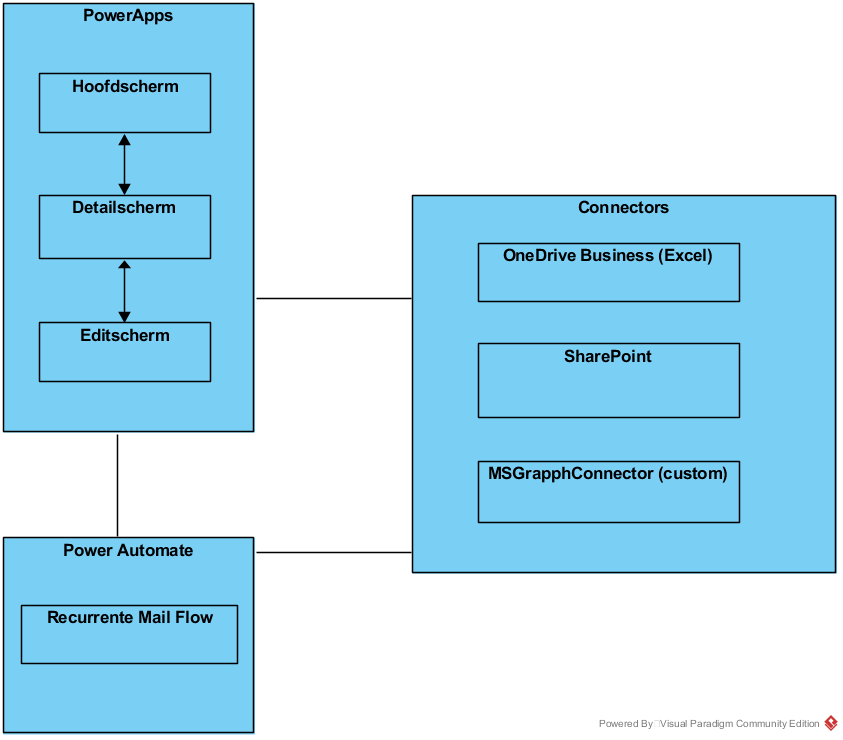
\includegraphics[width=0.8\linewidth]{PowerApps-POC-model.png}
    \caption{Model van de PowerApps proof-of-concept.}
    \label{fig:PowerApps-POC-model}
\end{figure}

\section{Requirements}

\subsection{Must have}

\subsubsection{Prijs}

Tijdens het maken van de POC werd gevonden dat de enige requirements die niet uitgewerkt kunnen worden met het de bestaande licentie het complex filteren en rapportage is (Custom Connector nodig). Indien er niet vanaf gedaan kan worden is er een aanvullend stand alone plan mogelijk. Dit houd in dat individuele gebruikers applicaties (2 apps en één portal) zonder functionaliteit beperkingen kunnen uitvoeren voor \euro 8.40 per maand\footnote{\url{https://powerapps.microsoft.com/en-us/pricing/}}. Deze app wordt door vier personen op de helpdesk gebruikt, dat brengt het totaal op \euro 33.60.

\begin{table}[h!]
    \begin{tabular}{|l|c|c|}
        \hline
        \textbf{PA met complexe functionaliteit} & \textbf{NEE} & \textbf{JA}             \\ \hline
        \textless{}= 2 apps                      & -            & \textgreater{}= \euro 33.60  \\ \hline
        \textgreater 2 apps                      & -            & \textgreater{}= \euro 134.40 \\ \hline
    \end{tabular}
    \caption{Meerprijs bovenop huidige licentie}
\end{table}

\subsubsection{Overzicht kunnen geven van belangrijkste info voor elk toestel in het netwerk}

Zoals reeds besproken in Sectie~\ref{sec:voorbereiding-pa} kan deze functionaliteit automatisch gegenereerd worden. Ook al is er voor tablet layout gekozen is het aantal realistisch weer te geven velden in het overzichtsscherm beperkt en werden de netwerknaam, omschrijving en dienst geselecteerd. Visuele indicatie van status was belangrijk in LanReview maar in plaats van de hele tekst van een rij in te kleuren is gekozen voor een gekleurd bolletje aan het hoofd van elke rij.\\
Data wordt aan de serverkant door SharePoint gevalideerd, het resultaat van deze validatie wordt getoond in de app zelf en dit is aangevuld met beperkte client side validatie. Dit komt neer op het aanwezig moeten zijn van de netwerknaam, het MAC-adres en device serial. In het detail- en edit scherm worden respectievelijk detailform en editform controls gebruikt. elk veld hierin wordt voorgesteld door een data card. Het is de 'required' eigenschap van een data-card die uitwijst of een veld ingevuld moet zijn.
% TODO: extra uitleg data cards + afb data card?

De flow van deze requirement wordt duidelijk aan de hand van het overzicht van navigaties tussen de schermen:\\
\begin{table}[h!]
    \begin{tabular}{|l|l|}
        \hline
        \textbf{Beweging}         & \textbf{Code}                                                   \\ \hline
        home $\rightarrow$ detail & \lstinline|Navigate(DetailScreen; ScreenTransition.None)|                   \\ \hline
        home $\rightarrow$ edit   & \lstinline|NewForm(Editform);;Navigate(EditScreen; ScreenTransition.None)|  \\ \hline
        home $\leftarrow$ detail  & \lstinline|Back()|                                                          \\ \hline
        detail $\rightarrow$ edit & \lstinline|EditForm(Editform);;Navigate(EditScreen; ScreenTransition.None)| \\ \hline
        detail $\leftarrow$ edit  & \lstinline|Back()|                                                          \\ \hline
    \end{tabular}
    \caption{Overzicht navigaties tussen schermen}
    \label{tab:app-flow}
\end{table}

\begin{figure}[h!]
    \centering
    \begin{subfigure}[b]{\linewidth}
        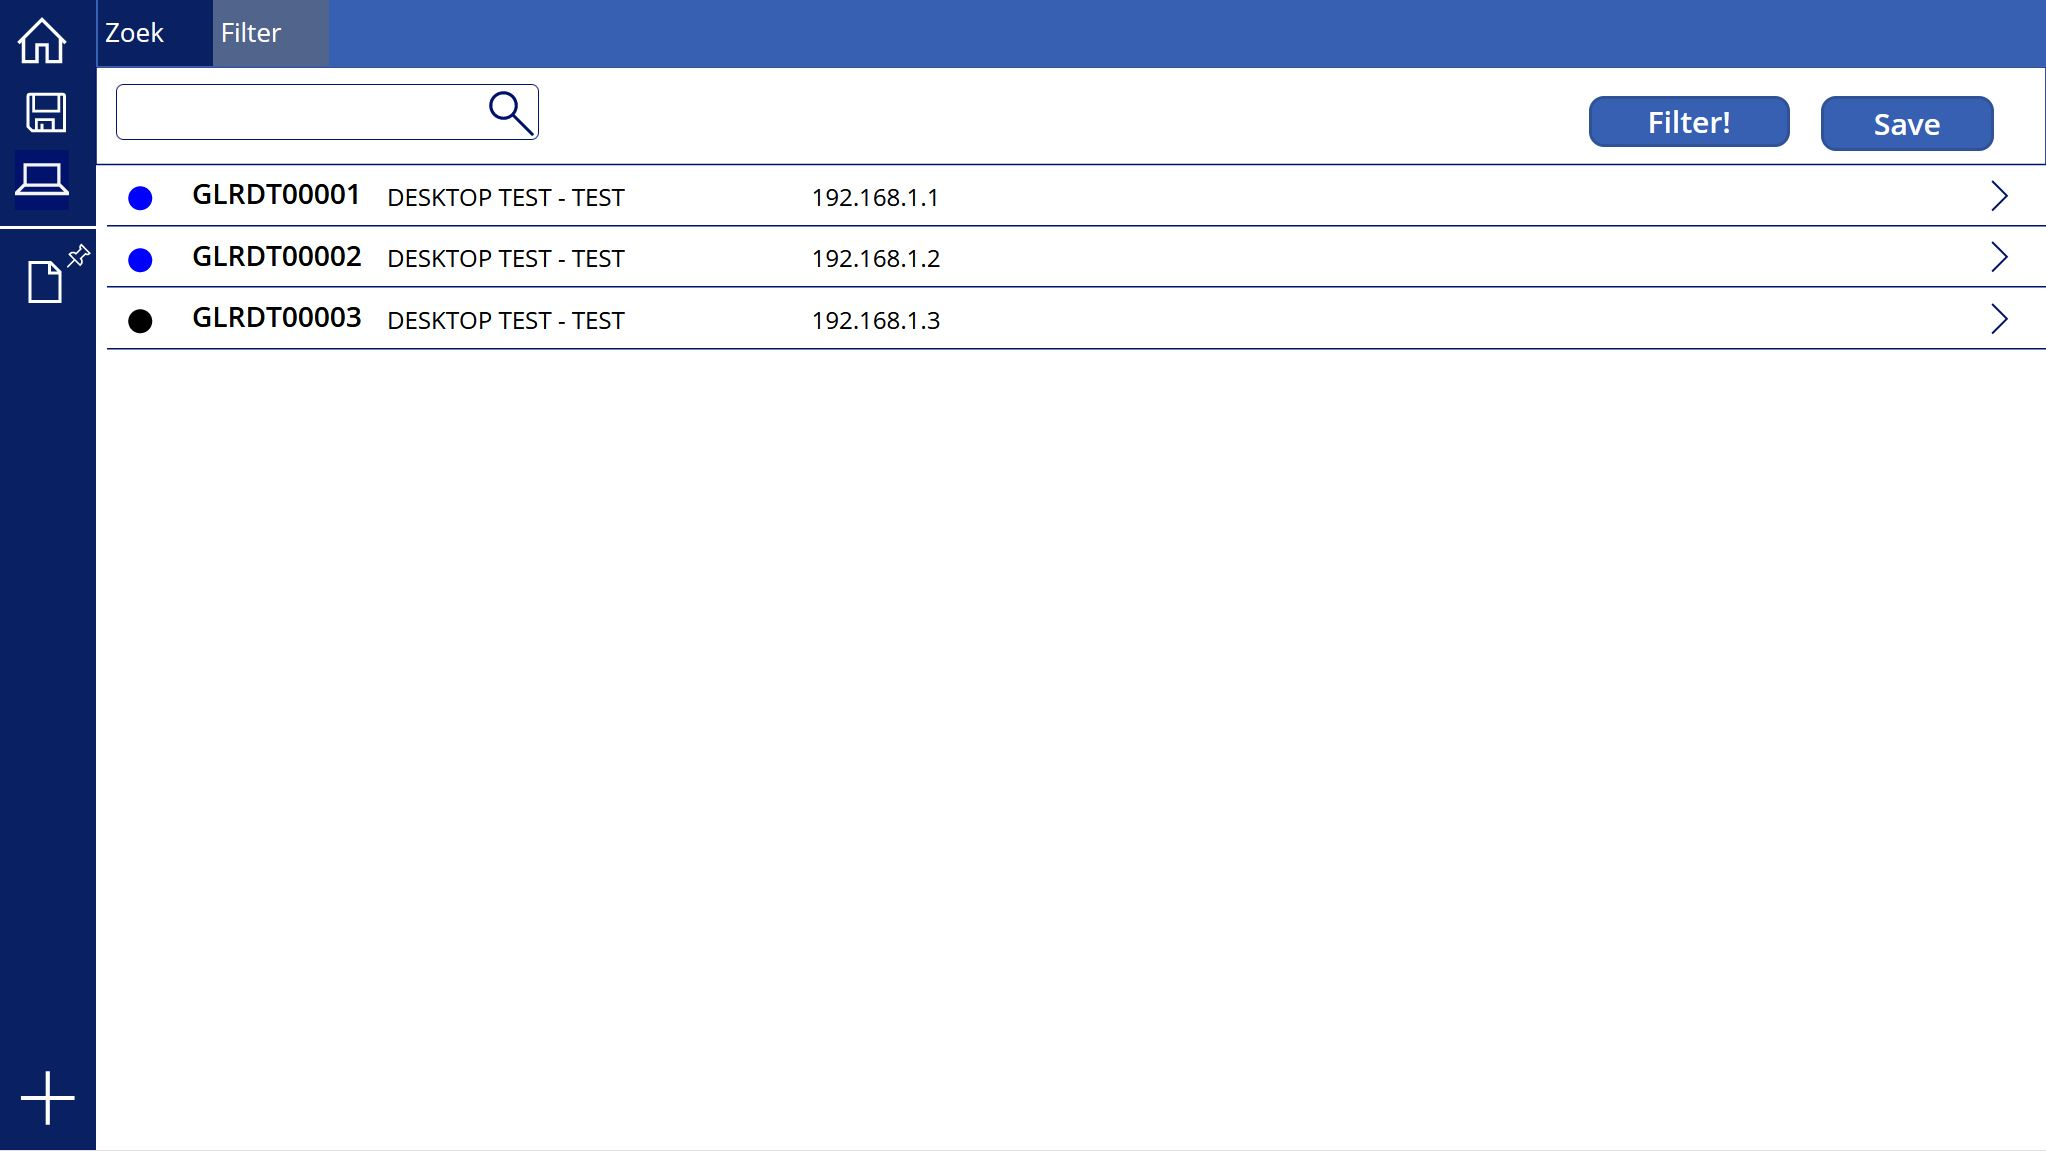
\includegraphics[width=\linewidth]{hoofdscherm-pa.JPG}
        \caption{Hoofdscherm}
    \end{subfigure}
    \begin{subfigure}[b]{\linewidth}
        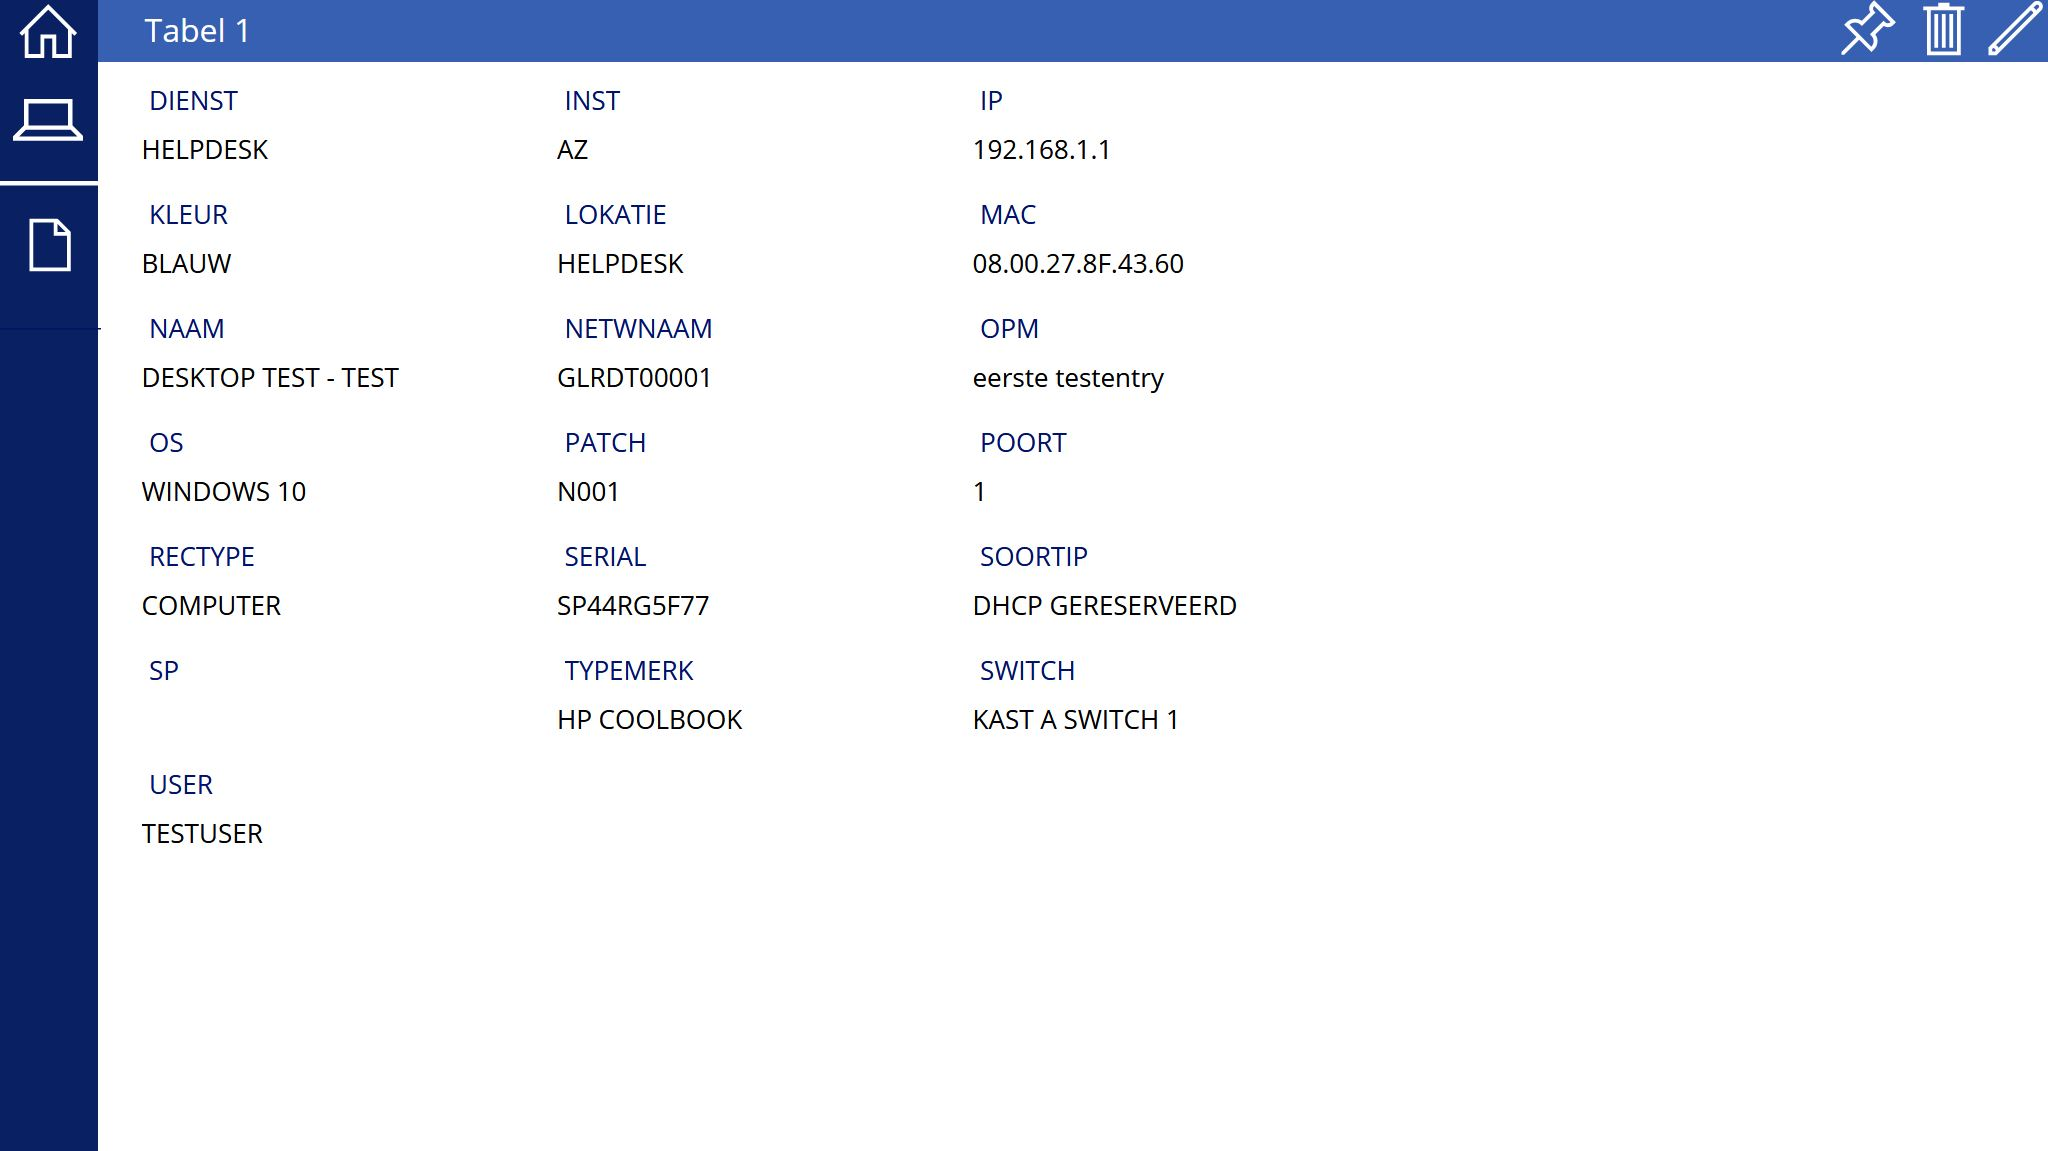
\includegraphics[width=\linewidth]{detailscherm-pa.JPG}
        \caption{Detailscherm}
    \end{subfigure}
    % \caption{overkoepelende caption}
    \label{fig:hoofd-detail-pa}
\end{figure}

\subsubsection{Filtering / rapportage}

\textit{Filtering (met Excel databron):}

Er moet een onderscheid gemaakt worden tussen 'zoeken' en 'filteren'. Zoeken is het matchen van tekst in een zoekveld aan een vooropgesteld aantal kolommen elke keer deze tekst wijzigt. Implementatie ervan in PowerApps is eenvoudig te doen met één formule:

\begin{lstlisting}
Search(Tabel1_1; SearchInput.Text; "NETWNAAM";"NAAM";"IP")
\end{lstlisting}

In geval van filtering moet het resultaat voldoen aan bepaalde condities. In PowerApps is een Filter formule aanwezig. Een voorbeeld implementatie kan zijn:

\begin{lstlisting}
Filter(Tabel1_1; MODEL = `HP COOLBOOK` && OS = `Windows 10`)
\end{lstlisting}

Dit oogt statisch. In LanReview is het mogelijk de kolom, operator en de filterwaarde in te stellen. Bovendien kunnen meerdere condities aaneengeschakeld worden.
Een gelijkaardige manier om filter data te verschaffen in PowerApps is door een gallerij te gebruiken waarbij elke rij een dropdown heeft voor de te filteren kolom, een dropdown voor het nodige vergelijkingsteken en een aan te passen tekstveld. Elke keer men een conditie toevoegt wordt deze data opgeslagen als rij in een Tabel.

% TODO: meer over de fitler werking in LanReview, filter doel
% TODO: afb!

Wat nu met mogelijkheden om de filter effectief uit te voeren? Er zijn een aantal opties, telkens met stijgende complexiteit.

\begin{enumerate}
    \item In PowerApps zelf met behulp van formules.\\
    Dit is niet mogelijk omdat we de te filteren kolom niet kunnen bepalen aan de hand van een variabele, er is geen string substitutie mogelijk. Het is ook niet mogelijk om het aantal condities dynamisch toe te wijzen (in het 'Filter' commando)).\\
    \textbf{$\rightarrow$ NEE}
    \item Via een Power Automate flow
    \begin{itemize}
        \item Filteractie `Een lijst maken met rijen in een tabel` (ODATA filter-query)\footnote{Filtering uitgelegd onder 'System Query Option \$filter' \url{http://docs.oasis-open.org/odata/odata/v4.0/errata03/os/complete/part2-url-conventions/odata-v4.0-errata03-os-part2-url-conventions-complete.html}}\\ 
            \textit{Wel:}  query kan als argument worden meegegeven.\\
            \textit{Niet:} 'and' operaties zijn niet ondersteund
         \item Filteractie `Matrix filteren` (flow expressie)\footnote{\url{https://docs.microsoft.com/en-us/power-automate/use-expressions-in-conditions}}\\
            \textit{Wel:} 'and' operaties zijn ondersteund\\
            \textit{Niet:} query kan niet als argument worden meegegeven.
    \end{itemize}
    \textbf{$\rightarrow$ NEE}
    \item Door gebruik van een Custom Connector.\\
    \textbf{$\rightarrow$ Ja}
    (zie Sectie~\ref{sec:custom-connector})
\end{enumerate}

Ter verduidelijking: een samengestelde query in zowel ODATA als flow expressie:
\begin{itemize}
    \item \textbf{ODATA:} \lstinline|(NETWNAAM eq 'GLRDT00001') and (IP eq '192.168.1.1')|
    \item \textbf{Flow expressie:} \lstinline|@and(equals(item()?['NETWNAAM'], 'GLRDT00001'),equals(item()?['IP'], '192.168.1.1'))|
\end{itemize}

Dit beoogde soort filtering is overigens out of the box aanwezig in model based apps. \autocite{MicrosoftDocs2020c}

Als het dynamische aspect van filtering opgegeven wordt is het nog steeds mogelijk om 'statisch' te werken. Daarmee bedoeld een aantal voorgebouwde queries, voor gangbare scenario's zoals ze bestaan in LanReview zijn zonder problemen op te nemen in PowerApps.

\textit{Filtering (met SharePoint databron):}

Filtering met SharePoint kan anders aangepakt worden, om dit aan te tonen worden de uitvoeringsopties opnieuw overlopen.
\begin{enumerate}
    \item In PowerApps zelf met behulp van formules.\\
    \textbf{$\rightarrow$ NEE}
    \item Via een Power Automate flow\\
    ODATA filters uitgevoert op SharePoint items hebben geen beperking op het aantal via 'and' aaneengekoppelde operaties, de filter kan dus in Power Automate uitgewerkt worden.\\
    \textbf{$\rightarrow$ JA}
\end{enumerate}

De belangrijkste operaties van de flow (Figuur~\ref{fig:sp-flow-open}) zijn:
\begin{itemize}
    \item \textbf{Items ophalen:} De ODATA filter query wordt als enkel string argument vanuit PowerApps doorgegeven naar de flow en is bruikbaar in het 'FilterQuery' veld.
    \item \textbf{Reactie:} Als eerst een test antwoord werd voorzien als voorbeeld om het schema uit te genereren wordt er een bruikbare json naar Powerapps teruggegeven.
\end{itemize}

\begin{figure}[h!]
    \centering
    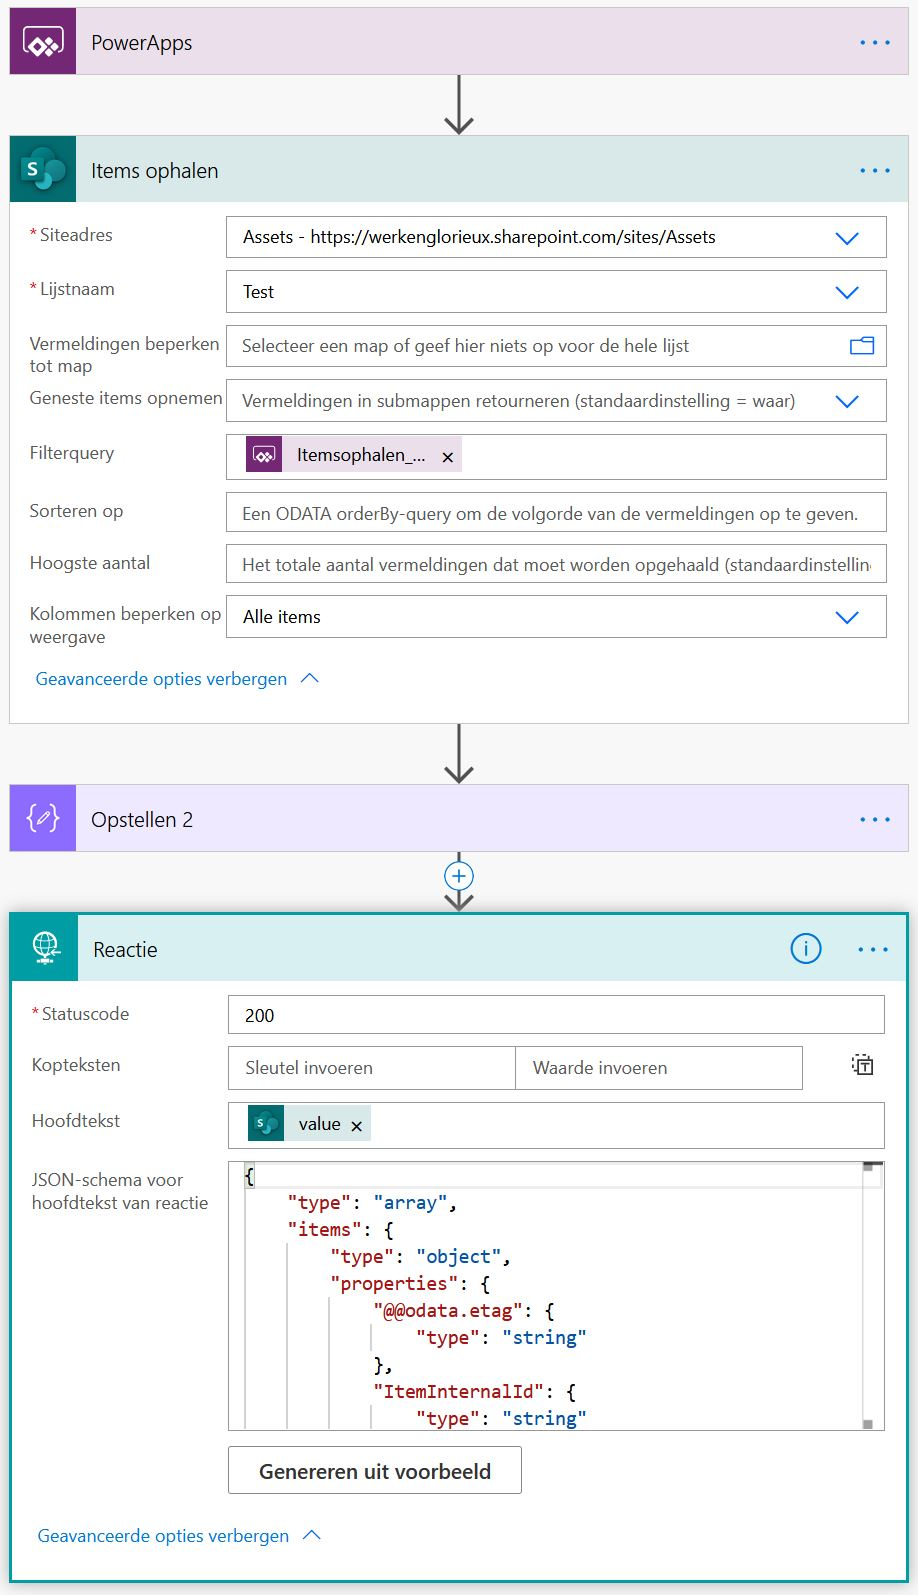
\includegraphics[width=0.8\linewidth]{sp-flow-open.JPG}
    \caption{De Automate flow waarmee SharePoint gefilterd wordt.}
    \label{fig:sp-flow-open}
\end{figure}

Gebruik in de PowerApp (Figuur~\ref{fig:sp-filter-res}):\\
De kolommen van SharePoint zijn enkel via een speciale soort naam toegankelijk, er moet mapping gebeuren. Daarvoor wordt een tabel gebruikt waarbij 'colPA' de kolomnaam is voor weergave in de PowerApp en 'colAUT' de bruikbare kolomnaam is in Automate.
\begin{lstlisting}
Set(ColNamesTable;Table({colPA:"NETWNAAM";colAUT:"Title"};{colPA:"NAAM";colAUT:"yh3z"};[..])) // entries voor eerste twee kolommen getoond.
\end{lstlisting}
Elke keer op 'formatquery' geduwd wordt:
\begin{lstlisting}
OnSelect => Collect(FormattedQueryHTTP;LookUp(ColNamesTable;colPA = colNameDropdown_1.SelectedText.Value).colAUT & " " & LookUp(OperatorsTable;eqPA = eqNameDropdown_1.SelectedText.Value).eqAUT & " '" & FilterValueText_1 & "'")
\end{lstlisting}
De waarden worden gemapt naar odata aanvaardbare waarden (via lookup), aan elkaar geplakt en toegevoegd aan tabel FormattedQueryHTTP als een enkelvoudige filter operatie.\\
Wanneer de query uitgevoerd wordt ('dynquery' knop):
\begin{lstlisting}
OnSelect => Set(HTTPFilterResults;'PowerApps-knop'.Run(Left(Concat(FormattedQueryHTTP;Value & " and ");Len(Concat(FormattedQueryHTTP;Value & " and "))- 5)))
\end{lstlisting}
De waarden van de tabel worden geconcateneerd met ' and' ertussen. De laatste 'and' wordt ervan gehaald via \lstinline|len(.., -5)|. De flow wordt uitgevoerd.

\begin{figure}[h!]
    \centering
    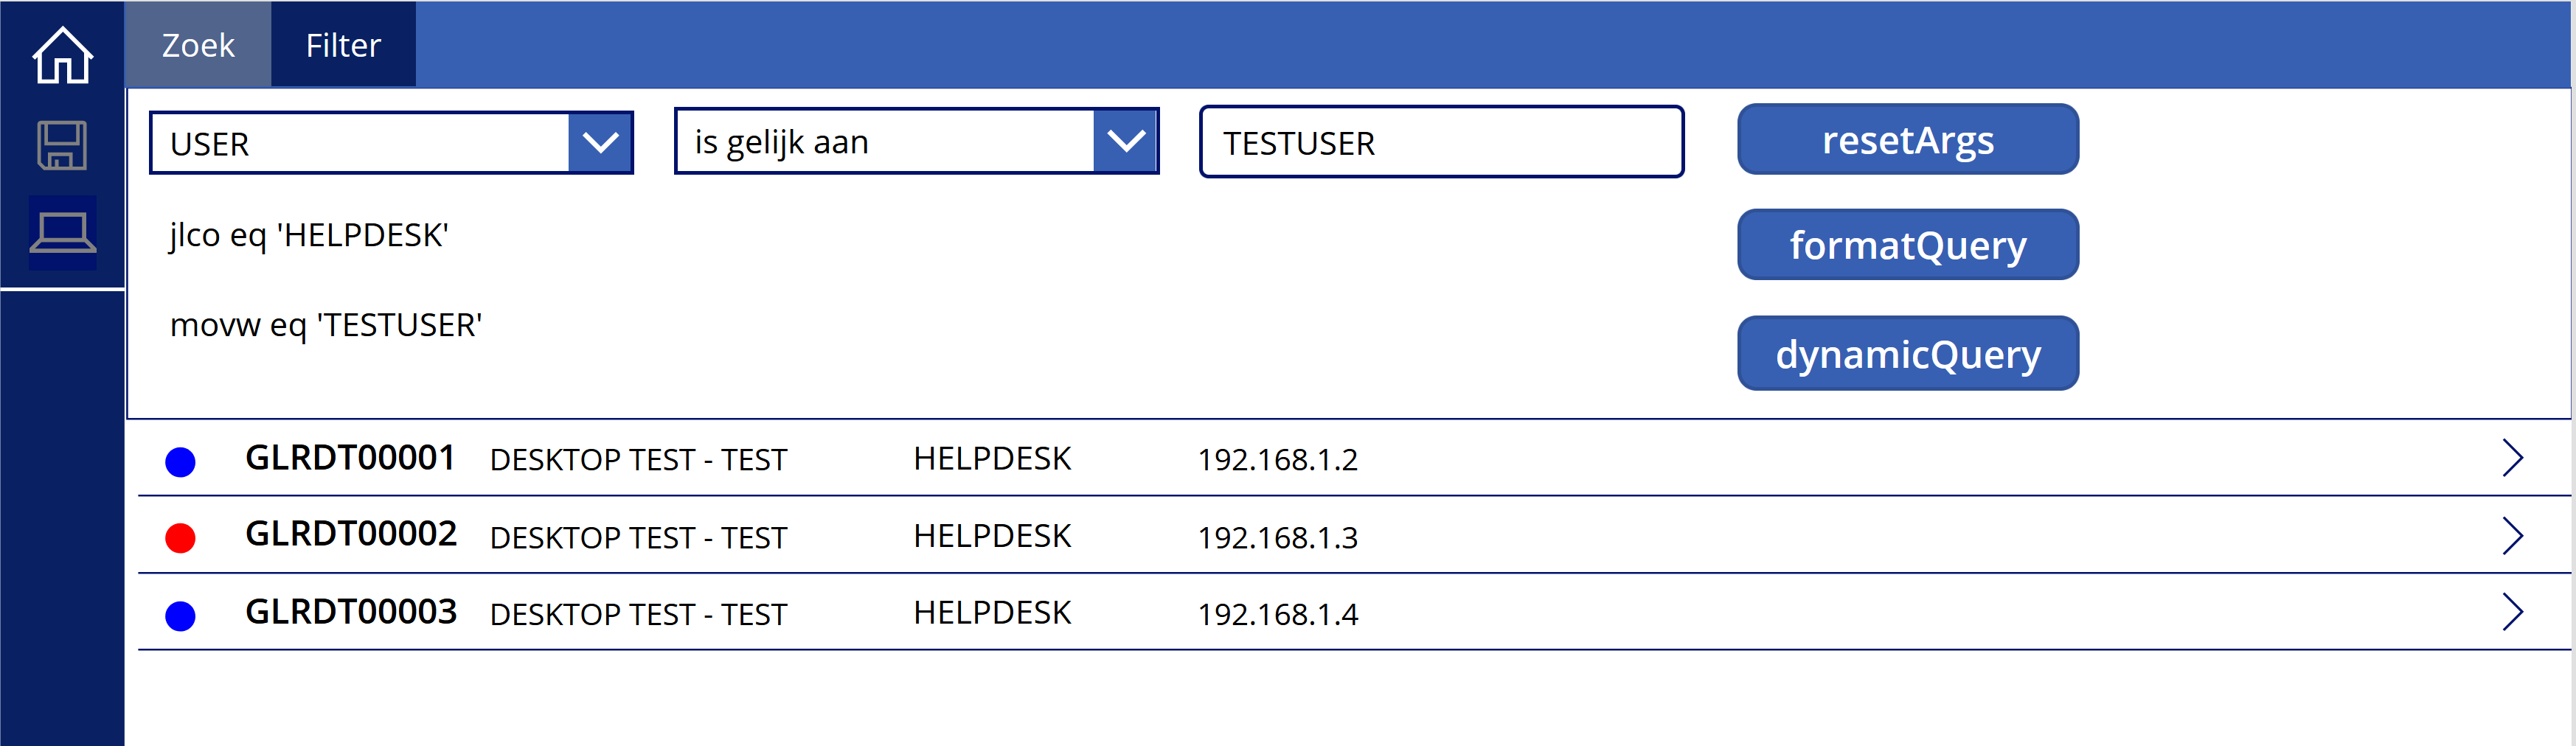
\includegraphics[width=\linewidth]{sp-filter-res.png}
    \caption{Voorbeeld van SharePoint filtering in de PowerApp.}
    \label{fig:sp-filter-res}
\end{figure}

\textit{Reporting:}

Het is niet mogelijk om data met een Power App lokaal op te slaan. De workaround is om de resultaten weg te schrijven naar een Excel in OneDrive dat specifiek dient voor reporting.

\subsubsection{Remote Desktop/Ping}
\label{subsec:rdp-ping}

Dit stelt een probleem. In LanReview is het mogelijk te rechtsklikken op een item en een remote desktop sessie te beginnen of een eenvoudige ping uit te voeren. Achter de schermen wordt dit als met de command prompt uitgevoerd. In Powerapps is het om te beginnen niet mogelijk om te rechtsklikken. Custom code uitvoering is standaard niet ondersteund. Zelf een custom connector bied hier geen oplossing omdat de app in de cloud leeft en aan serverzijde uitvoeren van RDP of ping heeft geen nut. Er is een workaround nodig.

PowerApps heeft een SaveData() methode om lokaal data op te slaan. Een typisch scenario is dat er geen internet is, app bewerkingen kunnen tijdelijk lokaal opgeslagen worden om definitief uit te werken als gedetecteerd wordt dat er terug internetverbinding is. Een eerste logische beperking is dat de SavaData() niet benaderbaar is buiten PowerApps, een tweede beperking is dat deze functionaliteit niet mogelijk is wanneer de app in een webbrowser en niet in een smartphone/tablet gebruikt wordt. Het idee om een IP-adres naar een configuratiebestand weg te schrijven om dan buiten de PowerApp te gebruiken om naar een pc te RDP'en of pingen stopt hier.

Het is mogelijk om een data gateway op te zetten. Dit zorgt voor een verbinding met on-premises data. Dit stelt een actie beschikbaar in Power Automate waarmee een bestand lokaal aangemaakt kan worden. Via een workaround kan er PowerShell mee uitgevoerd worden. \autocite{Luca2017}\\
Hier is niet voor gekozen om deze redenen: extra kosten, resource gebruik en configuratie voor een in verhouding kleine use case. Bovendien zou de data gateway ingesteld moeten worden op een gedeelde locatie, anders zou deze data gateway op de pc van elke PowerApp gebruiker moeten staan.

Een deel van het hierboven staande is bruikbaar, namelijk het idee om het IP-adres van de te pingen/rdp'en toestel voor te bereiden op een pc lokaal zodat de laatste stap manueel uitgevoerd kan worden. Dit moet in een bestandsformaat zijn waar Power Apps vlot mee overweg kan. Excel is een optie.

De uitwerking wordt:\\
In OneDrive een Excel file aanmaken met een kolom voor elke gebruiker van de app. De header waarde is  de voornaam van de gebruiker. Er is maar één rij aanwezig waar per kolom het huidige te pingen/rdp'en ip adres in staat. Instellen dat dit bestand lokaal gesynchroniseerd wordt (OndDrive is standaard Windows 10 functionaliteit).

De gebruiksflow is:
\begin{enumerate}
    \item Het detailscherm openen van de beoogde pc.
    \item Op de knop duwen om het ip adres weg te schrijven.
\begin{lstlisting}
OnStart => Set(Gebruiker;First(Split(User().FullName;" ")).Result)
OnSelect => Patch(iptable;First(Filter(iptable;user = Gebruiker));{ ip: SelectedDevice.IP})
\end{lstlisting}
    De formule gekoppeld aan 'OnStart' haalt de volledige naam van de ingelogde PowerApps gebruiker op en splitst deze waarna enkel het eerste resultaat (voornaam) wordt opgeslagen als 'Gebruiker' variabele.\\
    De formule gekoppeld aan het 'OnSelect' property haalt het IP-adres uit het detailformulier op en schrijft het weg naar de Excel tabel 'iptable' onder de kolom met de matchende gebruikersnaam.
    \item Lokaal kan nu een script uitgevoerd worden dat dit Excel bestand inleest en het relevante commando uitvoert (keuze hiervan hangt af van de overeenkomende snelkoppeling).
\begin{lstlisting}[style=powershellStyle]
$excelpad = "C:\Users\Thomas\OneDrive - Hogeschool Gent\rdpping_ips.xlsx"
$iptable = Import-Excel -Path $excelpad
$ip = $iptable.Where({$_.user -eq $env:USERNAME}).ip

if($args[1] -eq "ping"){
ping $ip
}elseif($args[1] -eq "rdp"){
Start-Process "$env:windir\system32\mstsc.exe" -ArgumentList "/v:$ip"
}else{
// extra commando
}
\end{lstlisting}
    Het 'import-excel' commando is mogelijk met de ImportExcel module\footnote{\url{https://github.com/dfinke/ImportExcel}}\\
    Voor het gemak wordt de uitvoering van het nodige commando gedaan via een snelkoppeling, de verwijzingen zijn:
\begin{lstlisting}
ping => C:\Windows\System32\WindowsPowerShell\v1.0\powershell.exe -NoExit -command "& 'H:\Documenten_TOSH\HoGent_Docs\2019-2020\Batchelorproef\C# apps\localtools.ps1' -commando ping"
RDP => C:\Windows\System32\WindowsPowerShell\v1.0\powershell.exe -NoExit -command "& 'H:\Documenten_TOSH\HoGent_Docs\2019-2020\Batchelorproef\C# apps\localtools.ps1' -commando rdp"
\end{lstlisting}
\end{enumerate}

Het nadeel is dat door deze extra overhead er 3-5 seconden gewacht moet worden voor het bestand gesynchroniseerd is en de nodige snelkoppeling uitgevoerd kan worden met het juiste IP-adres.

\subsubsection{Mobiel bruikbaar zijn}

Een Power App is onafhankelijk van platform of devicetype maar er wordt bij creatie wel gevraagd op welke layout er gefocust zal worden en het is zo dat de app er te groot of te klein uit zal zien als de app later gebruikt wordt op het toesteltype waar het niet voor ontworpen werd.\\
Om deze reden werd er een versie van de app gemaakt specifiek voor mobiel gebruik met een beperkte functionaliteitsset (Figuur~\ref{fig:pa-mobile}). Deze app zal voornamelijk gebruikt worden om snel een overzicht op te vragen van de belangrijkste info van een pc en om het toevoegen van nieuwe toestellen te vergemakkelijken met barcode scanning functionaliteit.

\begin{figure}[h!]
    \centering
    \begin{subfigure}[b]{0.45\linewidth}
        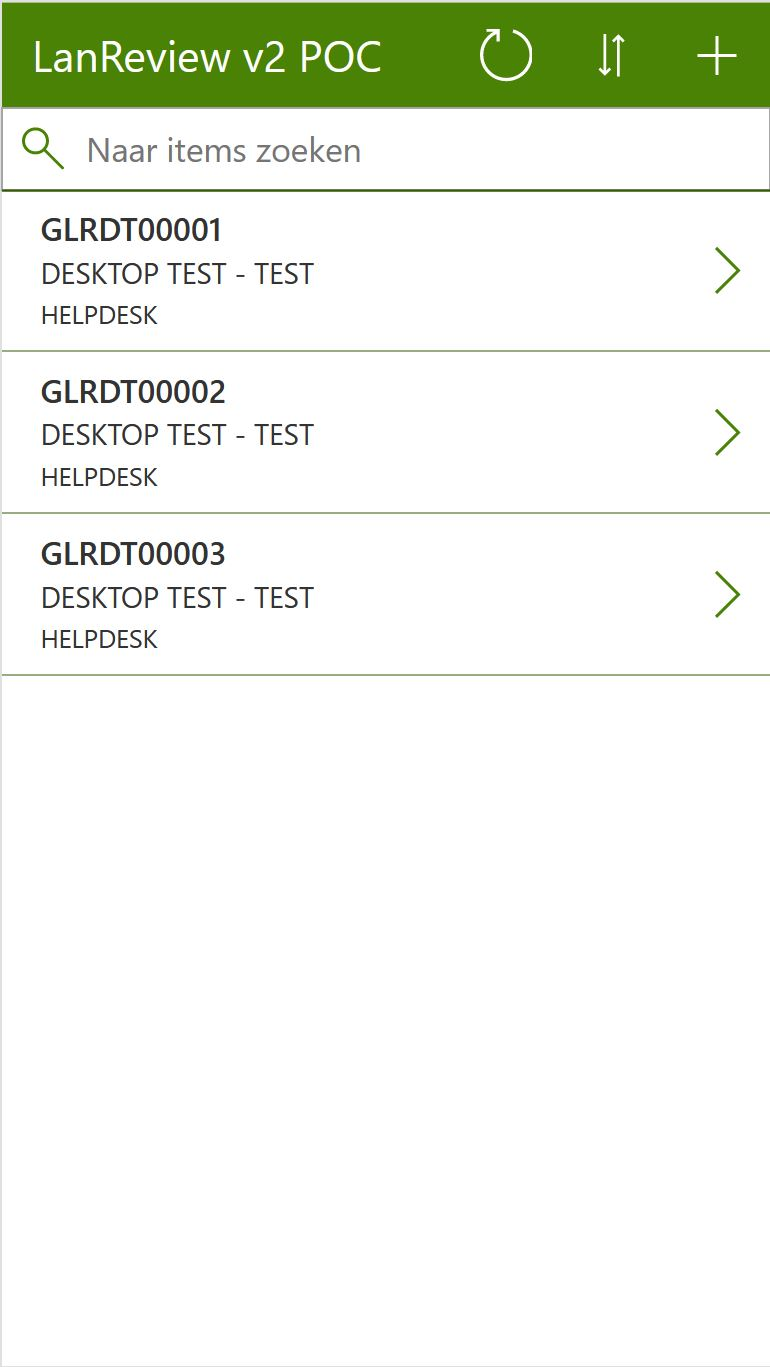
\includegraphics[width=\linewidth]{pa-mobile-hoofd.JPG}
        \caption{Hoofdscherm}
    \end{subfigure}
    \begin{subfigure}[b]{0.45\linewidth}
        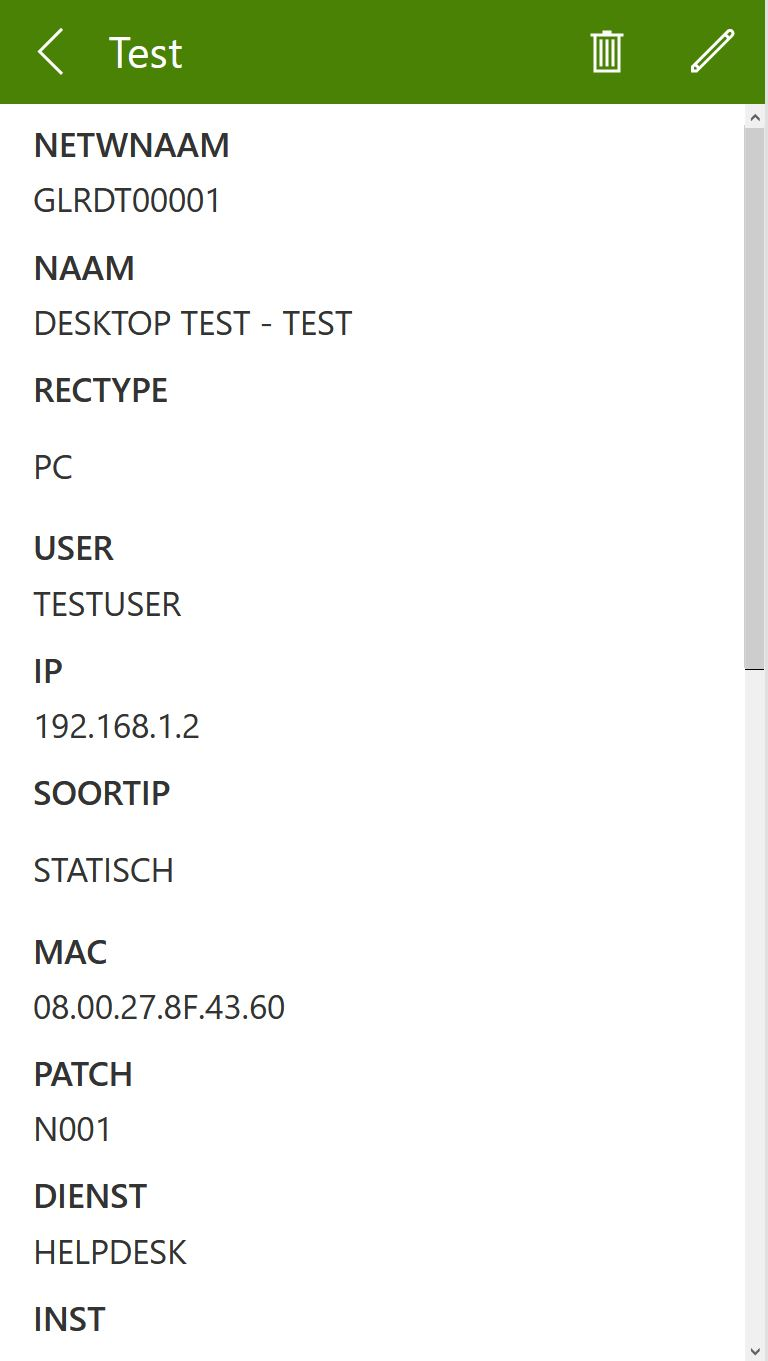
\includegraphics[width=\linewidth]{pa-mobile-detail.JPG}
        \caption{Detailscherm}
    \end{subfigure}
    \caption{Overzicht van de beperktere mobiele PowerApps POC}
    \label{fig:pa-mobile}
\end{figure}

\subsubsection{Future proof zijn}

Zowel \textcite{Rymer2019} als \textcite{Vincent2019} stelden dat klanten de licentiëring van producten in het Power platform verwarrend vonden. Hierboven komt dat deze licentiëring onderhevig kan zijn aan verandering \autocite{Pohl2019}.\\
Microsoft is een sterke aanwezigheid maar hetzelfde kan niet altijd gezegd worden over hun aangeboden producten \autocite{Bott2018}\\
De low-code markt is nog steeds turbulent volgens het eerder aangehaalde reports.
Als gekeken wordt naar de cyclische aard van low-code en de voorgangers beschouwd worden (vb, COBOL, 4GL, RAD ) stelt de vraag zich of dit vroeg of laat ook voorbij gestreefd zal worden? \autocite{Reselman2018}

\subsubsection{Performant zijn}

Een cloud applicatie die een lijst gebruikt in SharePoint of een Excel file in OneDrive zal niet even performant zijn als een lokale applicatie die een lokale Access databank gebruikt. Er zijn echter een aantal technieken om data operaties te optimaliseren zoals data voorladen met 'ClearCollect', calls parallel uitvoeren met 'ConcurrentCall' en laden van data voor niet zichtbare UI controls uitstellen met de 'Delayed Load' optie. \autocite{Andaloussi2018}\\
Er is nodige inefficiëntie geïntroduceerd in de app door gebruik van workarounds, bijvoorbeeld (subsectie~\ref{subsec:rdp-ping})\\
Er is kritiek dat gegenereerde code niet even geoptimaliseerd kan zijn als specifiek geschreven code. \autocite{Shiah2018}\\
Een belangrijke aanpassing die gemaakt moet worden is om de app 2000 kolommen op te laten halen in plaats van de standaard ingestelde 500. Er zijn meer dan 1000 toestellen en zoek en filteroperaties zouden anders maar op de eerste 500 toegepast worden.

\begin{figure}[h!]
    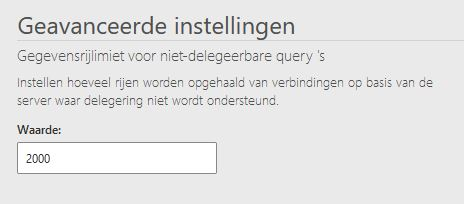
\includegraphics[width=0.7\linewidth]{2000-rows.JPG}
    \caption{Instelling voor aantal op te halen rijen}
    \label{fig:2000-rows}
\end{figure}

\subsubsection{Security}

% TODO:laatste controle
Eens een app gepubliceerd is kan gekozen worden wie de app mag gebruiken. Dit kan ook op groepsniveau gebeuren door te publiceren naar een bepaalde Environment. Goedgekeurde gebruikers hebben toegang met hun Office365 login, authenticatie gebeurt met andere woorden via Azure AD. Er moet opgepast worden dat deze gebruikers over de nodige permissies beschikken voor de aanwezige connectors om ontbrekende functionaliteit te vermijden.

Er zijn enkele technieken om granulaire permissies in te stellen, die van \textcite{Dunnam2019} wordt hier uitgelegd:

\textbf{Scenario:} Enkel bepaalde gebruikers mogen een formulier aanpassen.\\
\textbf{Toepassing:} Een (SharePoint) lijst opslaan met de email adressen van de gebruikers met bevoegdheid. Bij app start controleren of men in deze lijst zit. In de app zal de edit knop enkel maar voor hun zichtbaar zijn.\\
\textbf{Concreet:} 
\begin{lstlisting}
OnStart => ClearCollect(acceptedApprovers, Filter(Approvers, Title = User().FullName))
Visibkle (editknop) => If(IsEmpty(acceptedApprovers),false, true)
\end{lstlisting} 

Bovenstaande werd niet ingewerkt maar iets dergelijk zou later gebruikt kunnen worden om de app open te stellen voor een groter publiek (buiten enkel de IT).

\subsection{Should have}

\subsubsection{Gerichte/basis taken kunnen automatiseren}

De belangrijkste case hiervoor is dat er een wekelijks overzicht met toestellen moet rondgestuurd worden die langer dan een maand de status 'te schrappen' gekregen hebben, gekenmerkt door een 'KLEUR' veld met waarde 'BLAUW'. Een toestel krijgt de 'te schrappen' status wanneer ze verwijderd/vervangen worden uit de actieve omgeving en in opslag worden geplaatst. Het is dan de gewoonte om een maand te wachten voor een toestel effectief verwijdert wordt (in geval van ontbrekende data of een functioneel probleem in de nieuwe oplossing).\\
Dit is als flow geïmplementeerd, zie Figuur~\ref{fig:flow-sharepoint-kort}

\begin{figure}[h!]
    \centering
    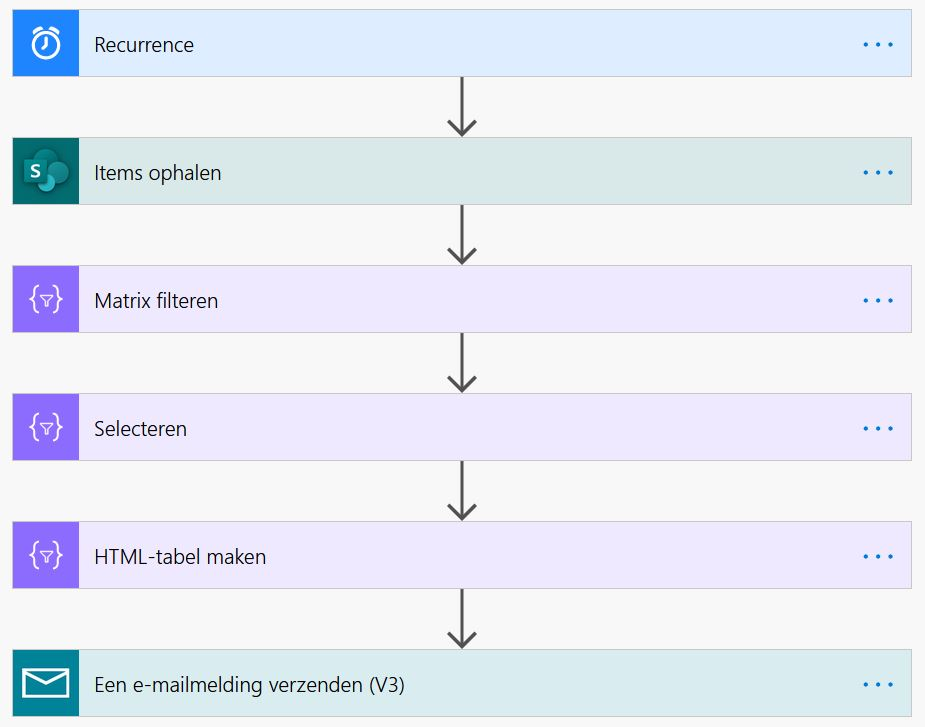
\includegraphics[width=0.7\linewidth]{flow-sharepoint-kort.JPG}
    \caption{Recurrente flow met SharePoint databron.}
    \label{fig:flow-sharepoint-kort}
\end{figure}

Er is ook een flow uitgewerkt met Excel als databron. Het verschil is dat een datum wordt teruggegeven als integer en dat enkele formules aangepast moeten worden om hier mee om te gaan (Figuur~\ref{fig:recurrent-flow-excel}). 

\begin{figure}[h!]
    \centering
    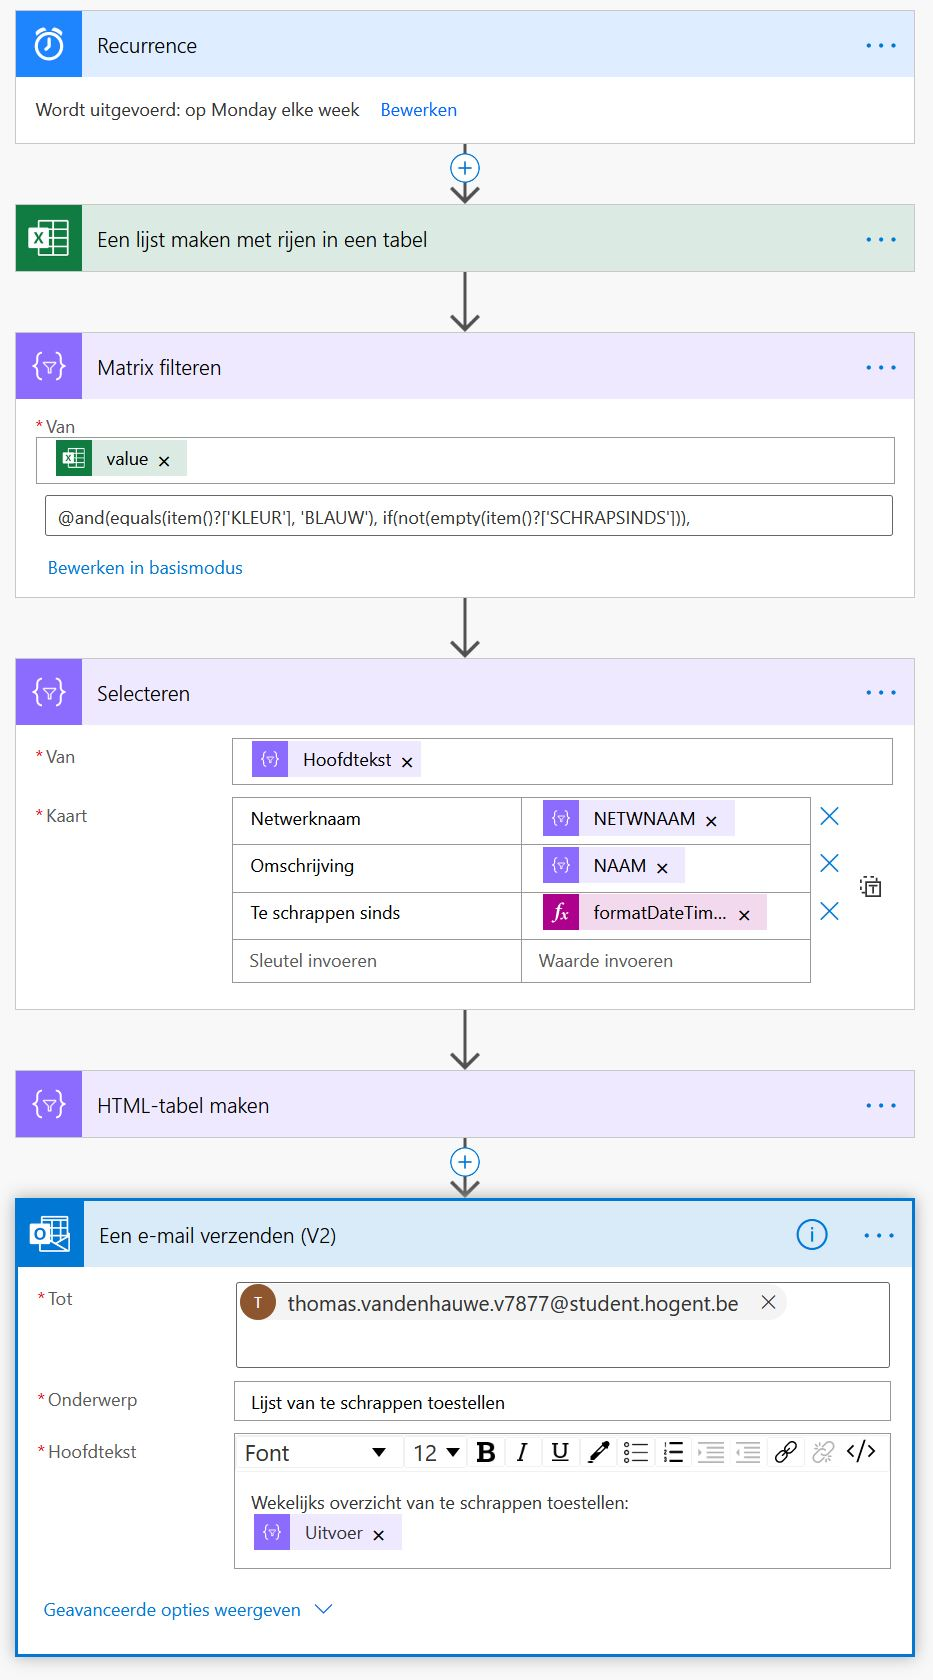
\includegraphics[width=0.7\linewidth]{afb-herhaalde-flow.JPG}
    \caption{Recurrente flow met Excel databron.}
    \label{fig:recurrent-flow-excel}
\end{figure}

\begin{enumerate}
    \item \textbf{Recurrence:} Het is een recurrente flow. Het tijdschema is wekelijks, maandag om 3.00u.
    \item \textbf{Een lijst maken met rijen in een tabel:} In deze stap worden de rijen uit de nodige Excel tabel enkel opgehaald, filtering gebeurt in de volgende stap. Er wordt dus niet met ODATA gefilterd maar via flow expressies.
    \item \textbf{Matrix filteren:} Om te voldoen moet KLEUR BLAUW zijn, het SCHRAPDATUM veld mag niet leeg zijn en moet een datum bevatten van meer dan een maand geleden.
\begin{lstlisting}
SharePoint => @and(equals(item()?['b0et']?['Value'], 'BLAUW'), if(not(empty(item()?['SCHRAPDATUM'])), lessOrEquals(item()?['SCHRAPDATUM'], addDays(utcNow(), -31)), false))
Excel => @and(equals(item()?['KLEUR'], 'BLAUW'), if(not(empty(item()?['SCHRAPSINDS'])), lessOrEquals(addDays('1899-12-30', int(item()?['SCHRAPSINDS'])), addDays(utcNow(), -31)), false))
\end{lstlisting}
    Excel geeft datums terug als integers van het aantal dagen sinds 1900. Als dit toegevoegd wordt aan '1899-12-30' is de correcte datum terug opgesteld en kan dit vergeleken worden met de huidige datum \lstinline|utcNow()|. Dit werd besproken in de PowerApps forums\footnote{\url{https://powerusers.microsoft.com/t5/Building-Flows/Excel-Online-Date/td-p/134200}}
    \item \textbf{Selecteren:} De in de mail te gebruiken kolommen uit het resultaat van de filter halen. Zo kunnen ze gebruikt worden in de volgende stap.
    \item \textbf{HTML-tabel maken:} Het resultaat van de vorige stap wordt als argument opgegeven. Er wordt een html tabel opgesteld.
    \item \textbf{Een e-mail verzenden (V2):} Het reële adres zal dat van de helpdesk zijn. In de body van de mail kan de HTML-tabel ingevoegd worden.
\end{enumerate}

Het resultaat is dat iedereen op de helpdesk automatisch een mail krijgt met het overzicht. Figuur~\ref{fig:flow-result}

\begin{figure}[h!]
    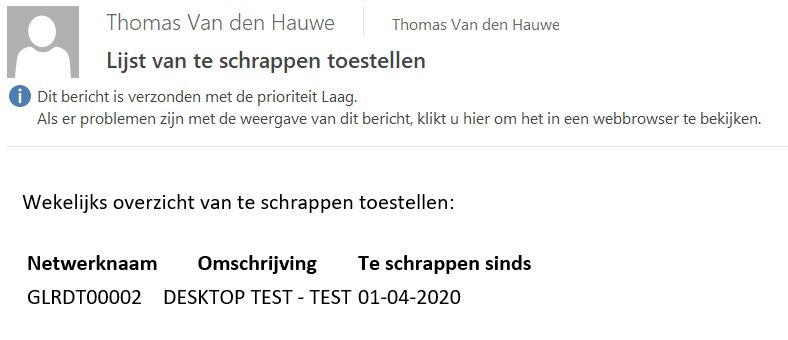
\includegraphics[width=0.7\linewidth]{flow-result.JPG}
    \caption{Een voorbeeld van de mail.}
    \label{fig:flow-result}
\end{figure}

% TODO: extra cases

\subsubsection{Bruikbaar zijn buiten domein}

De app leeft in de cloud. Het enige dat nodig is zijn geldige Office365 credentials en een internetverbinding.

\subsubsection{SharePoint requirements}

Requirements die met SharePoint te maken hebben zijn:
\begin{itemize}
    \item Nieuwe types toestellen opnemen.
    \item Randapparatuur opnemen.
    \item Revisie van elk dataveld per toesteltype.
    \item Data opslaan in SharePoint (cloud).
\end{itemize}
Deze worden besproken in Sectie~\ref{sec:sharepoint}

\subsubsection{Leercurve moet degelijk zijn}
\textit{(Dit deel is gebaseerd op persoonlijke ervaringen van de auteur)}

\begin{itemize}
    \item \textbf{Uiterlijk $\rightarrow$ Gemakkelijk:} Uiterlijk is eenvoudig te configureren met drag-en-drop. layout eigenschappen moeten niet vaak aangepast worden doordat controls in positie 'springen'. Groepen visuele controls kunnen gekopieerd en geplak worden.
    \item \textbf{Data en variabelen $\rightarrow$ Opletten:} Data gebruik kan uitdagend zijn indien niet goed ingepland. Gebruik van variabele is eenvoudig maar het overzicht erover kan verloren gaan omdat ze gedeclareerd worden bij het eerste gebruik
    \item \textbf{Gedrag en uitbreidingen $\rightarrow$ Moeilijk:} Gedrag instellen is moeilijk, formules hebben een leercurve. Uitbreidingen schrijven is ook moeilijk, voorkennis van REST principes was nodig.
\end{itemize}

Als een case out of the box ondersteund is op PowerApps zal een business gebruiker er geen problemen mee hebben. Zeker niet als ze voorkennis van Excel hebben.

\subsection{Nice to have}

\subsubsection{Samenwerken met SCCM en/of synchroniseren met en data uit de SQL databank kunnen gebruiken}

% TODO: meer utileg over script in bron
Dit werd niet geïmplementeerd maar er is wel een mogelijke oplossing voor gevonden.
In essentie gaat het om een script dat volgens een tijdschema uitgevoerd wordt op de SCCM server dat SCCM cmdlets gebruikt om asset data op te vragen die weggeschreven worden naar een SharePoint omgeving.\autocite{Ziehnert2020}

Het vorige betreft synchronisatie, Alternatief kan een de AdminService REST API gebruikt worden om rechtstreekse toegang te krijgen tot SCCM data vanuit PowerApps of Automate. \autocite{Gross2019}\\
De configuratie hiervan valt buiten de scope van het onderzoek, de grote stappen illustreren dit:

SMS Provider API (SCCM) $\rightarrow$ SMS Provider rol (site server) $\rightarrow$ Cloud Management Gateway $\rightarrow$ certificaat $\rightarrow$ Azure App registratie $\rightarrow$ Custom Connector

In de POC zijn er bovendien geen requirements die nood hebben aan directe toegang tot SCCM en de Custom Connector brengt extra kosten mee.

\subsubsection{Diverse GUI verbeteringen/robuust GUI ontwerp ondersteunen}

% [[afb-toolbar-muis-over-pin][afb-pin-detailscreen]

Het is mogelijk items vast te pinnen op de toolbar. Toevoegen gaat door rechtsboven op het 'pin' symbool te klikken in de detailweergave van een pc. losmaken van de toolbar is analoog door op de rode 'pin' rechtsboven van het icoon te klikken. Als gehovered wordt over de toolbar wordt de Netwerknaam ook getoond. (Figuur~\ref{fig:toolbar-pin-clipped})

\begin{figure}[h!]
    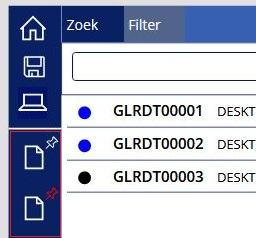
\includegraphics[width=0.5\linewidth]{toolbar-pin-clipped.jpg}
    \caption{Een voorbeeld van vastpinnen aan de toolbar.}
    \label{fig:toolbar-pin-clipped}
\end{figure}

Voor duidelijkheid zijn de zoek in filter velden van elkaar gescheiden door tabs. Tabs worden gemaakt met Gallerij controls.

De filter layout is ook gemaakt met een Gallerij control. De layout past zich dynamisch aan als er filtervelden worden toegevoegd. (Figuur~\ref{fig:filter-clipped})

\begin{figure}[h!]
    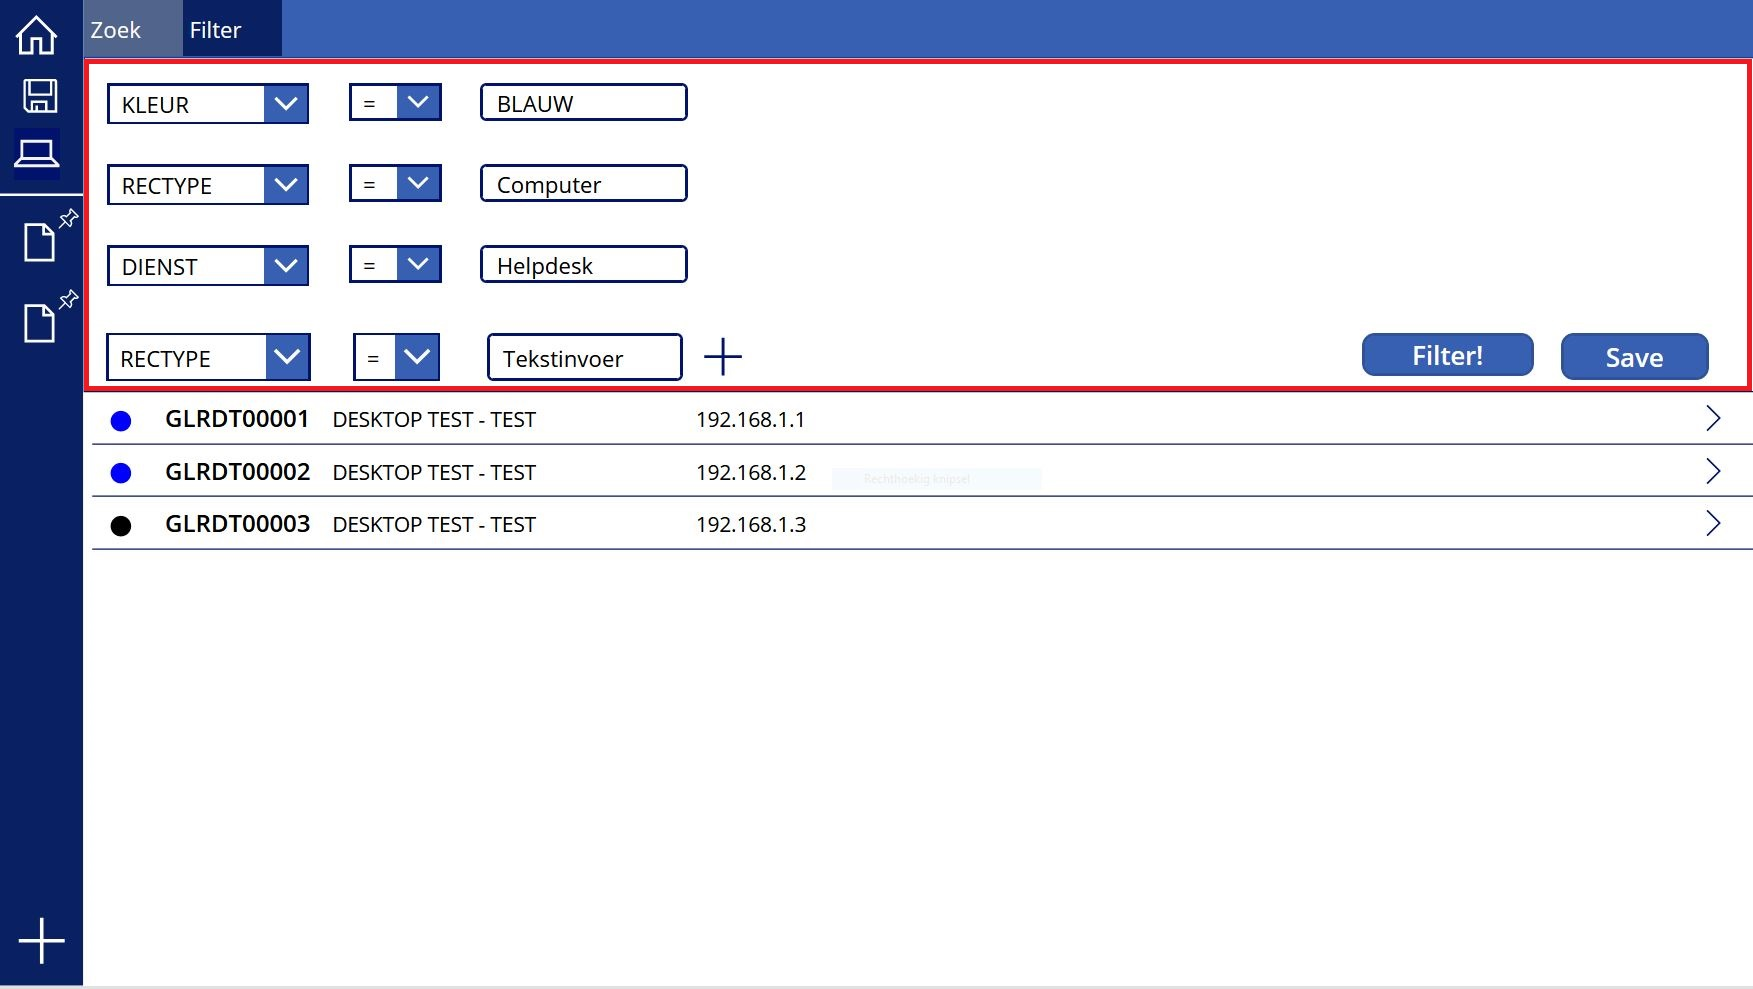
\includegraphics[width=\linewidth]{filter-clipped.jpg}
    \caption{Dynamisch aanpassen van layout aan filter condities.}
    \label{fig:filter-clipped}
\end{figure}

\subsubsection{Barcodes kunnen scannen}

Er is een control beschikbaar specifiek om barcodes in te scannen. Dit maakt het proces om deze functionaliteit toe te voegen aan de app zo eenvoudig als het aanmaken van een Label. Er dient dus geen speiale connector toegevoegd of geconfigureerd te worden. Standaard kan deze scanner enkel gebruikt worden op een tablet of smartphone maar via de instellingen kan een alternatieve webbarcodescanner gekozen worden.

Het gebruiksscenario is dat men tijd wil besparen bij het toevoegen van nieuwe toestellen door de barcode en serial in te scannen in plaats van manueel over te typen (en de kans op fouten te vergroten). Toestellen worden soms in bulk aangekocht dus de potentiële tijdswinst is aanzienlijk.

Dit is geïmplementeerd door een barcode knop toe te voegen aan de MAC en SERIAL data cards in het editscherm. Indien er op de klop geduwd word opent de camera, word de barcode waarde uitgelezen en toegevoegd aan het relevante tekstveld.\\
Ondersteunend moeten maar twee property waarden aangepast worden.
\begin{itemize}
    \item Button $\rightarrow$ OnScan: Als de scanner gebruikt werd wordt de uitgelezen waarde toegevoegd aan een context variabele.
\begin{lstlisting}
UpdateContext({ScannedMac: BarcodeScanner1.Value})
\end{lstlisting}
    \item TextField $\rightarrow$ Default: Als er een ScannedMac variabele aangemaakt werd wordt deze als tekst gebruikt in plaats van de standaard waarde.
\begin{lstlisting}
If(IsBlank(ScannedMac);Parent.Default;ScannedMac)
\end{lstlisting}    
\end{itemize}

\subsubsection{AI functionaliteit}

Er werd geen enkele requirement opgesteld die AI nodig zou hebben maar de mogelijke opties werden toch even verkend.

Zoals reeds besproken werd in Subsectie~\ref{subsec:recente-wijzigingen} zijn er verschillende opties. Via AI Builder kan een model getraind worden of kan een voorgebouwd model gebruikt worden voor een typisch scenario. Gebruik van AI Builder is prijzig (\euro 421.70 per unit/maand), er is een calculator\footnote{\url{https://powerapps.microsoft.com/nl-nl/ai-builder-calculator/}} om exacte berekeningen te maken. Een alternatief is om AI functionaliteit te introduceren aan de hand van een specifieke connector.\\
Een eenvoudige voorbeeldcase die zo'n connector gebruikt (bijvoorbeeld Azure Computervision\footnote{\url{https://azure.microsoft.com/nl-nl/services/cognitive-services/computer-vision/}}) is om het Netwerknaam uit te lezen van de label die op een PC plakt met tekstherkenning. Indien het aantal API calls beperkt blijft is het gebruik van deze connector bovendien gratis.
% TODO: ndoige connector acties invoegen

\section{Custom Connector}
\label{sec:custom-connector}

Een Custom Connector is de enige optie om code of een niet ondersteunde databron te introduceren in PowerApps. Er zijn twee varianten onderzocht:
\begin{itemize}
    \item Azure API App (Swagger definitie)
    \item Blank Custom Connector
\end{itemize}
Het doel is om een complexe filter uit te werken. Een eerste idee was om alle data naar de API te posten en de filtering binnen de app zelf uit te werken. Hier werd snel vanaf gestapt naar de Microsoft Graph API. %(Zie Subsectie~\ref{subsec:ms-graph})


\subsection{Microsoft Graph}
\label{subsec:ms-graph}

\begin{figure}[h!]
    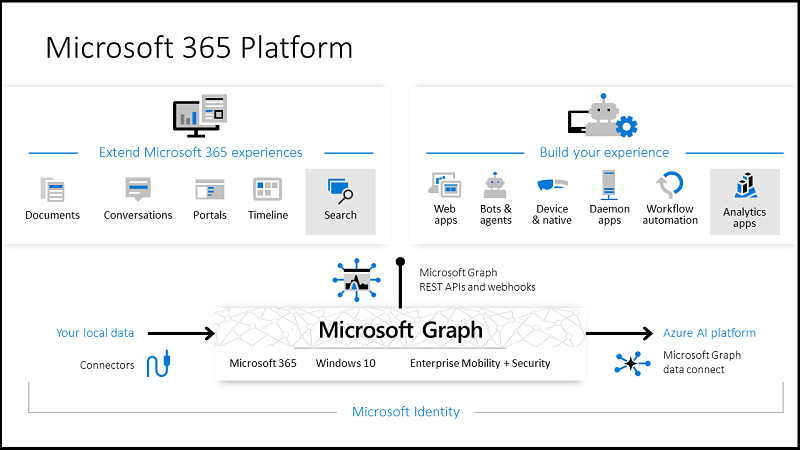
\includegraphics[width=\linewidth]{ms-graph.png}
    \caption{Microsoft Graph in het Microsoft 365 platform \autocite{MicrosoftDocs2020d}}
    \label{fig:ms-graph}
\end{figure}

% info ms graph uitbreiden

Microsoft Graph is een REST\footnote{REpresentational State Transfer \url{https://restfulapi.net/}} API waarmee allerhande data uit Office365 services opgevraagd kan worden. De specifieke case is het filteren van Excel data in OneDrive.\\
Een volgt een overzicht van de nodige stappen en bijbehorende requests om dit te verwezenlijken.
In dit eenvoudige voorbeeld wordt gefilterd op een pc met Netwerknaam 'GLRDT00001'. Niet relevante header waarden zijn weggelaten.
\begin{enumerate}
    \item Een sessie creëren in de Excel file met data. Dit is nodig om de filter effectief toe te kunnen passen in stap 3. In de response body is de sessie-id te vinden.
\begin{lstlisting}
POST https://graph.microsoft.com/v1.0/me/drive/root:/testdata.xlsx:/workbook/createsession
BODY => {persistChanges:true}
\end{lstlisting}
    \item Reeds bestaande filters verwijderen moesten deze nog aanwezig zijn.
\begin{lstlisting}
POST https://graph.microsoft.com/v1.0/me/drive/root:/testdata.xlsx:/workbook/worksheets('Blad1')/tables('tabel1')/clearFilters
\end{lstlisting}
    \item De filter toepassen. De sessie-id moet meegegeven worden als header waarde. In de URL is de kolomnaam te vinden `columns('NETWNAAM')'. De operator en eigenlijke filterwaarde staan in de request body '"criterion1": "=GLRDT00001"'.
\begin{lstlisting}
POST https://graph.microsoft.com/v1.0/me/drive/root:/testdata.xlsx:/workbook/worksheets('Blad1')/tables('tabel1')/columns('NETWNAAM')/filter/apply
HEADER => workbook-session-id: {session-id}
BODY => 
{
"criteria" : 
    { "filterOn": "custom",
    "criterion1": "=GLRDT00001"
    }
}
\end{lstlisting}
    \item Het resultaat van de filter opvragen. Enkel de 'values' tag volstaat, daarom wordt er op gefilterd in de visibleView met 'rows?\$select=values'
\begin{lstlisting}
GET https://graph.microsoft.com/v1.0/me/drive/root:/testdata.xlsx:/workbook/worksheets('Blad1')/tables('tabel1')/range/visibleView/rows?$select=values
\end{lstlisting}
\end{enumerate}


\subsection{Azure API App (ASP.NET)}

Via Microsoft Graph is er toegang tot de data maar nu is er vanuit de Power Apps zelf toegang nodig tot Microsoft Graph. De optie die de meeste vrijheid bied is het maken van een .NET API in Visual Studio, dit wordt naar Azure gedeployed (als Azure API App) en later geïmporteerd in PowerApps als Custom Connector aan de hand van een Swagger definitie. Er is ook de keuze of de app gebouwd wordt in ASP.NET framework of .NET Core. Om praktische redenen werd gekozen om de ASP.NET framework variant te maken, het is namelijk mogelijk om de nodige Azure app registratie vanuit Visual Studio zelf uit te voeren.
In .NET zijn er aantal klassen beschikbaar waarmee Microsoft Graph bewerkingen uitgevoerd kunnen worden waarvan de belangrijkste 'GraphServiceClient' is. Het gebruik ervan wordt verder uitgelegd.

\textit{Voorbereiding: Azure App registratie}

\begin{figure}[h!]
    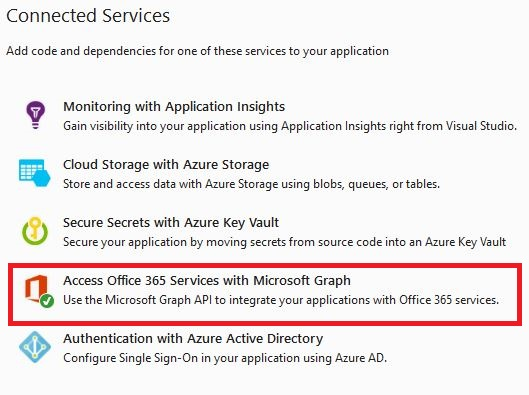
\includegraphics[width=0.7\linewidth]{vs-connected-services.JPG}
    \caption{Microsoft Graph in de Connected Services}
    \label{fig:vs-connected-services}
\end{figure}

In de solution staat in de 'Connected services' lijst een optie om te verbinden met Office365 services via de Microsoft Graph (Figuur~\ref{fig:vs-connected-services}). In deze wizard wordt een nieuwe Azure App registratie aangemaakt (indien nog niet bestaand) en kunnen de nodige permissies aan de hand van 'scopes' bepaald worden. De scopes om OneDrive bestanden te kunnen gebruiken zijn:
\begin{itemize}
    \item User.Read 
    \item Files.Read 
    \item Files.Read.All 
    \item Files.ReadWrite 
    \item Files.ReadWrite.All
\end{itemize}

Na afloop zijn zijn er enkele belangrijke stukken gegevens ingevoegd in de Web.config, een korte verklaring:
\begin{itemize}
    \item \textbf{TenantId:} Identifier van de Active Directory gebruiker/tenant, ook de id van de map waar waar de resources zich bevinden.
    \item \textbf{ClientId:} Identifieert de app registratie in Active Directory.
    \item \textbf{ClientSecret:} Secret geassocieerd met de ClientId.
\end{itemize}

Nu kan er over gegaan worden op de implementatie. Er zijn twee technieken toegepast om de 'GraphServiceClient' klasse te configureren.\\
De eerste is gebaseerd op de techniek gevonden op CodeProject\footnote{Demystifying Microsoft Graph - \url{https://www.codeproject.com/Tips/5249834/Demystifying-Microsoft-Graph}}:
\begin{lstlisting}[style=CSharpStyle]
//
public static async Task<GraphServiceClient> GetGraphServiceClient()
{
var authentication = new
{
Authority = "https://graph.microsoft.com",
Directory = WebConfigurationManager.AppSettings["ida:TenantId"],
Application = WebConfigurationManager.AppSettings["ida:ClientId"],
ClientSecret = WebConfigurationManager.AppSettings["ida:ClientSecret"]
};

var app = ConfidentialClientApplicationBuilder.Create(authentication.Application)
.WithClientSecret(authentication.ClientSecret)
.WithAuthority(AzureCloudInstance.AzurePublic, authentication.Directory)
.Build();

var scopes = new[] { "https://graph.microsoft.com/.default" };

var authenticationResult = await app.AcquireTokenForClient(scopes)
.ExecuteAsync();

var graphServiceClient = new GraphServiceClient(
new DelegateAuthenticationProvider(x =>
{
x.Headers.Authorization = new AuthenticationHeaderValue(
"Bearer", authenticationResult.AccessToken);

return Task.FromResult(0);
}));
return graphServiceClient;
}
\end{lstlisting}

De tweede gebuikt een techniek beschreven op CSharpCorner\footnote{Integrate Microsoft Graph With .NET CORE Web APIs - \url{https://www.c-sharpcorner.com/blogs/integrate-microsoft-graph-with-net-core-web-apis}}:
\begin{lstlisting}[style=CSharpStyle]
//
public static async Task<GraphServiceClient> GetGraphServiceClient2()
{
var authentication = new
{
Authority = "https://graph.microsoft.com/",
Directory = WebConfigurationManager.AppSettings["ida:TenantId"],
Application = WebConfigurationManager.AppSettings["ida:ClientId"],
ClientSecret = WebConfigurationManager.AppSettings["ida:ClientSecret"],
GraphResourceEndPoint = "v1.0",
Instance = WebConfigurationManager.AppSettings["ida:AADInstance"],
Domain = WebConfigurationManager.AppSettings["ida:Domain"]
};
var graphAPIEndpoint = $"{authentication.Authority}{authentication.GraphResourceEndPoint}";
var newAuth = $"{authentication.Instance}{authentication.Directory}";
//var newAuth2 = $"{authentication.Instance}{authentication.Domain}";

AuthenticationContext authenticationContext = new AuthenticationContext(newAuth);
Microsoft.IdentityModel.Clients.ActiveDirectory.ClientCredential clientCred 
= new Microsoft.IdentityModel.Clients.ActiveDirectory
    .ClientCredential(authentication.Application, authentication.ClientSecret);
Microsoft.IdentityModel.Clients.ActiveDirectory.AuthenticationResult authenticationResult 
= await authenticationContext.AcquireTokenAsync(authentication.Authority, clientCred);
var token = authenticationResult.AccessToken;
var delegateAuthProvider = new DelegateAuthenticationProvider((requestMessage) =>{
requestMessage.Headers.Authorization = new AuthenticationHeaderValue("bearer", token.ToString());
return Task.FromResult(0);
});

var graphClient = new GraphServiceClient(graphAPIEndpoint, delegateAuthProvider);
return graphClient;
}
\end{lstlisting}

Het verschil tussen beide zit in de dependencies die gebruikt worden om een instantie van de 'GraphServiceClient' te bouwen. De stappen die ze uitvoeren echter zijn hetzelfde en kunnen als volgt beschreven worden:
\begin{enumerate}
    \item Nodige variabelen declareren voor onder andere de ClientId, TenantId, ClientSecret.
    \item De app/authenticatie(context) bouwen aan de hand van deze gegevens.
    \item Een token genereren
    \item Een instantie van GraphServiceClient aanmaken en returnen.
    %\item Deze instantie gebruiken om operaties uit te voeren op Microsoft Graph.
\end{enumerate}

Deze instantie wordt teruggegeven naar een Controller klasse (hier FilterController) waar de HTTP operaties in gedeclareerd worden. In onderstaand voorbeeld worden alle aanwezige items in OneDrive teruggegeven:
\begin{lstlisting}[style=CSharpStyle]
// GET api/values/5
public async Task<string> Get(string filter)
{
try
{
GraphServiceClient client = await MicrosoftGraphClient.GetGraphServiceClient2();
var resultaat = await client.Users["db4fef52-9274-49e2-846c-1f325c4b9d7c"].Drive.Root
    .Children.Request().GetAsync();

return resultaat.ToString();
}
catch (MsalUiRequiredException)
{
    //
\end{lstlisting}

Als bovenstaande test query uitgevoerd wordt via de Swagger UI wordt er een fout teruggegeven. (Zie Figuur~\ref{fig:swagger-error})
Het probleem is dat het hier aangemaakte soort token applicatie permissies in plaats van gedelegeerde permissies nodig heeft. Voor gedelegeerde permissies is een ingelogde gebruiker nodig. Applicatie permissies zijn in Azure enkel in te stellen met een Administrator account.

Het sjabloon\footnote{GitHub GraphSDK - \url{https://github.com/rogreen/GraphSDK/blob/master/GraphSDKDemo/Views/MainPage.xaml.cs}} uit de officiële Graph documentatie gebruikt deze soort token.\autocite{MicrosoftDocs2020d} Dit is echter niet mogelijk voor een API die in Power Apps opgeroepen moet worden. Er is een andere oplossing nodig.

\begin{figure}[h!]
    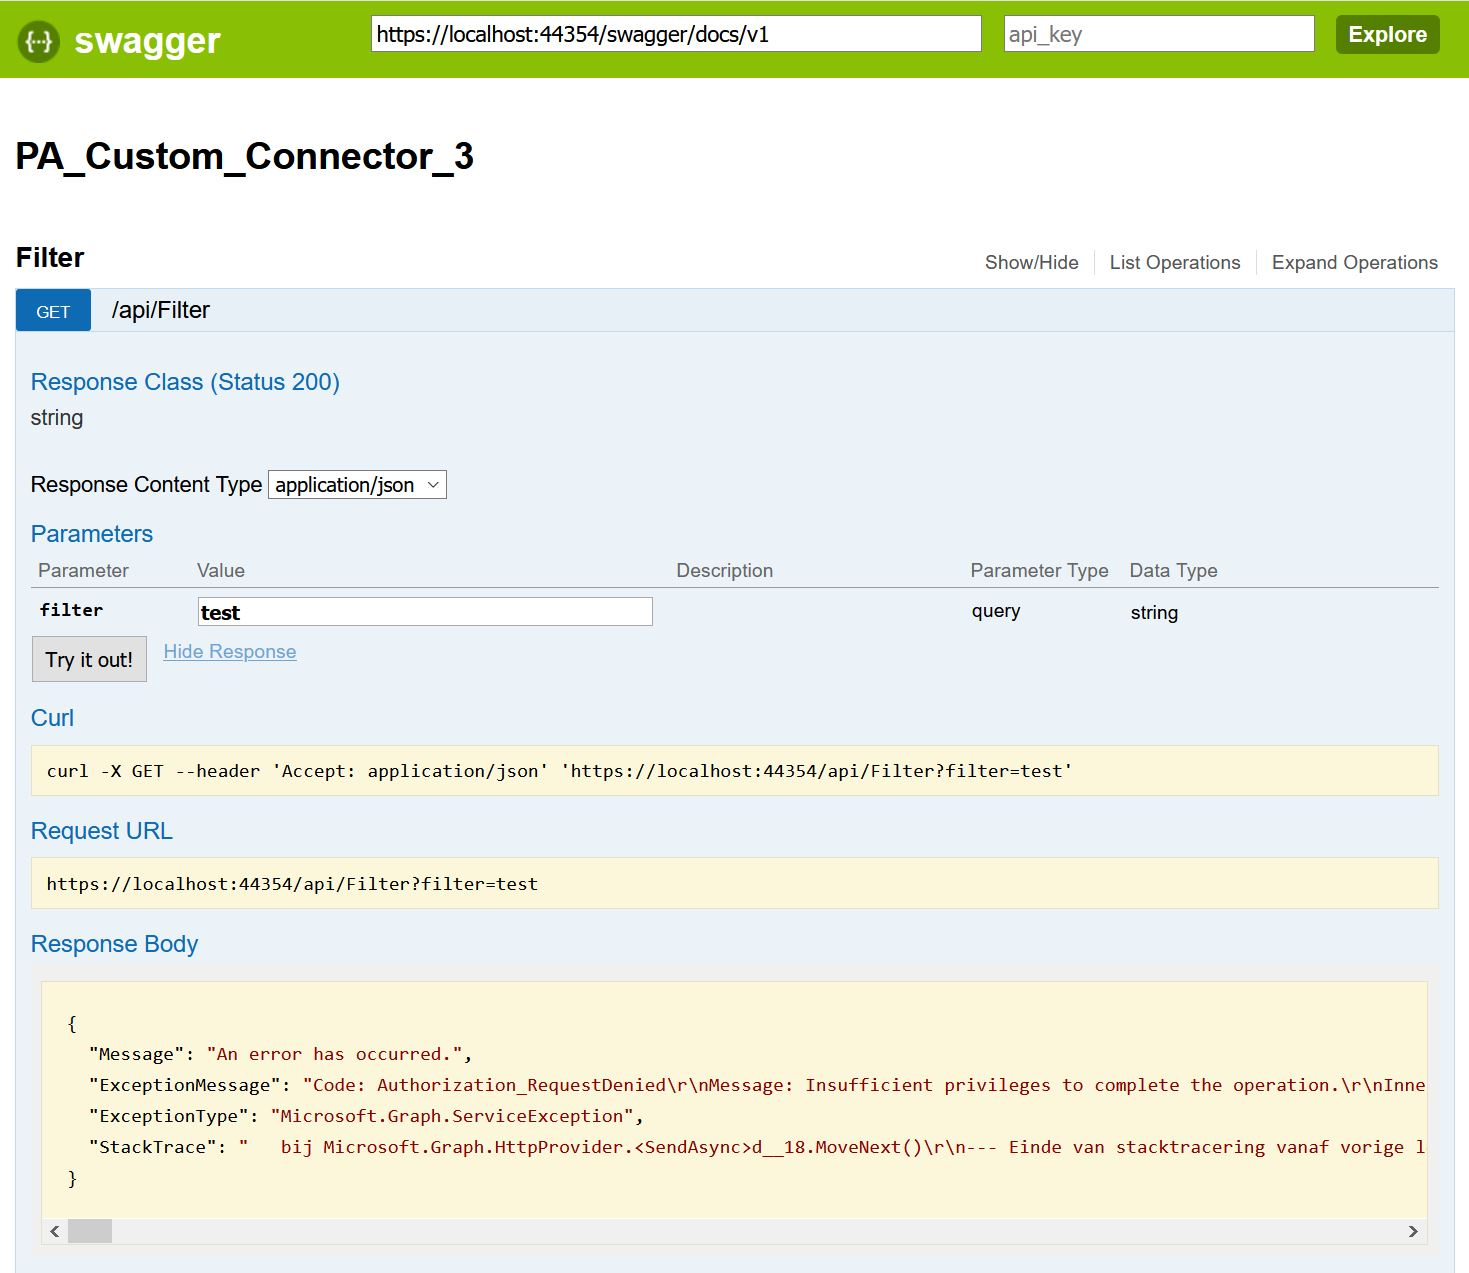
\includegraphics[width=\linewidth]{swagger-error.JPG}
    \caption{Teruggegeven error bij het maken van requests.}
    \label{fig:swagger-error}
\end{figure}

\subsection{Blank Custom Connector}

Er kan aangenomen worden dat als de Custom Connector in Power Apps zelf gemaakt wordt (via de optie 'Create from blank') en de nodige Microsoft Graph requests rechtstreeks gedeclareerd worden, dat de permissies van de ingelogde PowerApps gebruiker genomen worden om deze later uit te voeren, dat het ingevoegde soort token met andere woorden gedelegeerde permissies zal hebben.

Vergeleken met hoe het in de vorige sectie ging moeten de stappen in Azure manueel uitgevoerd worden.
%Vergeleken met hoe het in de vorige sectie ging moet de app eers manueel geregistreerd worden in Azure.
\begin{enumerate}
    \item Nieuwe app registratie maken.
    \item Een Client secret aanmaken.
    \item Scope permissies instellen, dit was: \lstinline|User.Read Files.Read Files.Read.All Files.ReadWrite Files.ReadWrite.All|
\end{enumerate}

Als nu de optie 'Create from blank' geselecteerd wordt start een wizard:\\ 
\textbf{General $\rightarrow$ Security $\rightarrow$ Definition $\rightarrow$ Test}

In het 'Security' tab is het belangrijk OAuth v2.0 authenticatie te kiezen met als id provider 'Azure Active Directory'. Dan komt het neer op het invullen van de gegevens die net in Azure aangemaakt zijn. Het echte werk begint in de 'Definitie' tab. De operaties uit Subsectie~\ref{subsec:ms-graph} werden eerst in Microsoft Graph Explorer\footnote{\url{https://developer.microsoft.com/en-us/graph/graph-explorer}} getest, hierna worden de request en response gegevens gebruikt om een actie te maken. Deze actie kan licht aangepast worden wat variabelen gebruik betreft zodat bijvoorbeeld de filterargumenten uit PowerApps correct kunnen doorgeven worden naar deze connector.\\
Het is handig dat in de laatste stap de acties getest kunnen worden. De resultaten hiervan zijn ingevoegd. (Figuur~\ref{fig:res-blank-conn})

\begin{figure}[h!]
    \centering
    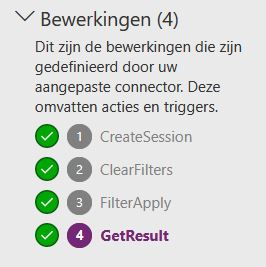
\includegraphics[width=0.4\linewidth]{res-blank-conn.JPG}
    \caption{Resultaat van de Graph queries.}
    \label{fig:res-blank-conn}
\end{figure}

In de PowerApp worden deze acties opgeroepen via formules gekoppeld aan de 'OnSelect' property van de 'Filter !' knop.
\begin{lstlisting}
Set(filterSessionID;MSGraphConnector.CreateSession({persistChanges:true}).id);;
MSGraphConnector.ClearFilters();;
ForAll(filterVelden;MSGraphConnector.FilterApply(veld.Value;filterSessionID;{filterOn:"custom";criterion1:gelijkTeken.Value & filterTekst}));;
Set(filterResultaatItems;MSGraphConnector.GetResult({'$select':"values"}).value);;
\end{lstlisting}
\begin{enumerate}
    \item Een Excel workbook sessie starten en de gereturnde id koppelen aan een variabele.
    \item Vorige filters verwijderen.
    \item Voor elke rij in de 'filterVelden' tabel wordt filter actie oproepen. De aanvaarde argumenten in volgorde zijn: kolomnaam, sessie id en een record waarin de stringwaarde van de operator en filterwaarde aan elkaar geplakt worden (via '\&').
    \item Er wordt een variable gedeclareerd dat het relevant stuk return json toegewezen krijgt via de 'GetResult' actie.
\end{enumerate}

Theoretisch ziet dit er goed uit, de tests ervoor slagen en de eerste actie geeft het sessie id succesvol terug. Jammer genoeg falen de andere. Er wordt telkens een 404 (resource not found) error teruggegeven.

De gevonden workaround is om de oproepen naar de Custom connector uit te laten voeren vanuit een flow. Figuur~\ref{fig:excel-filter-flow-success} toont de succesvolle uitvoering hiervan.

\begin{figure}[h!]
    \centering
    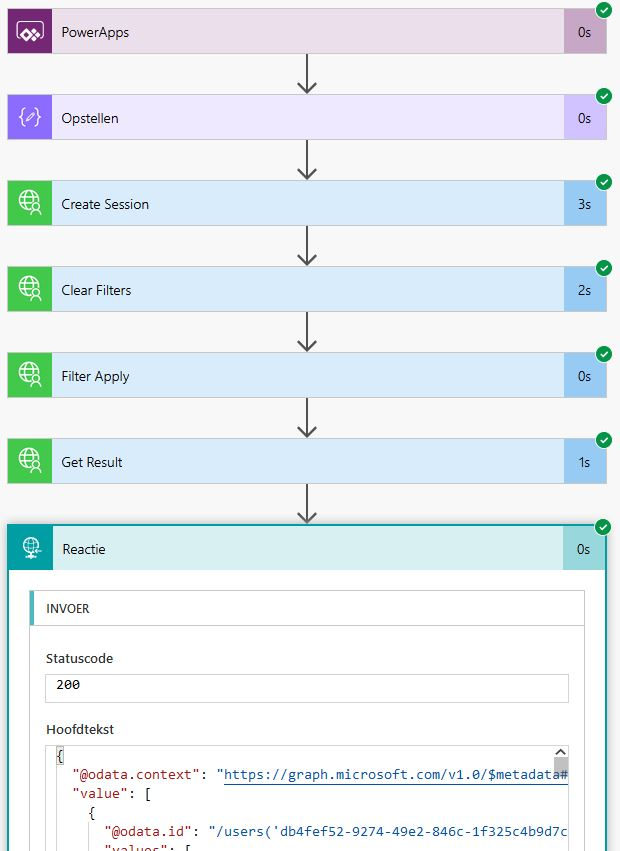
\includegraphics[width=0.8\linewidth]{excel-filter-flow-success.JPG}
    \caption{Gebruik van de Custom Connector in een flow, de acties van deze connector zijn groen.}
    \label{fig:excel-filter-flow-success}
\end{figure}

Enkele opmerkingen die het gebruik van de flow verduidelijken:\\
In de powerapps wordt de flow uitgevoerd via 'Filter !' knop.
De filterargumenten moeten als invoerparameters meegegeven worden. Deze moeten formatting krijgen.
De resultaten van 'GetResult' worden teruggestuurd in 'Reactie' en zijn als json toegankelijk vanuit de PowerApp mits het schema eerst gedefinieerd werd.
